\chapter{CƠ SỞ LÝ THUYẾT}
\label{chap:background}
\paragraph{Chương 2} trình bày các kiến thức nền tảng cần thiết phục vụ cho quá trình thực hiện đề tài, bao gồm các nội dung:

\begin{itemize}
\item Giới thiệu về mạng học sâu, một phạm trù của Machine Learning

\item Định nghĩa, cấu trúc, cách hoạt động của mạng neural nhân tạo

\item Mở rộng của mạng neural nhân tạo - mạng neural tích chập - cấu trúc, các lớp, cơ chế tính toán và ứng dụng của nó trong việc xử lí dữ liệu có dạng hình ảnh

\item Các thuật toán nhận diện hình ảnh sử dụng mô hình neural tích chập, gồm: R-CNN, Fast R-CNN và Faster R-CNN
\end{itemize}

\section{Giới thiệu về mạng học sâu (Deep Learning)}
Học máy (ML) là một lĩnh vực của Trí tuệ nhân tạo (AI) nhằm tập trung vào xây dựng các mô hình có thể học tự động từ dữ liệu cho sẵn để giải quyết những bài toán cụ thể. Một ví dụ điển hình là nhờ Học máy, một máy có thể tự động học được cách phân loại thư điện tử xem có phải là thư rác hay không. 

Ngày nay, ứng dụng của Học máy ngày càng đa dạng, phổ biến hơn nữa, bao gồm dịch tự động, nhận dạng tiếng nói, nhận dạng chữ viết, biển số xe, nhận dạng hình ảnh,... trong nhiều lĩnh vực khác nhau từ kinh tế, y học,... đến nông nghiệp. 

Học sâu (DL) thuộc một phạm trù của ML, là một kĩ thuật tập trung giải quyết vấn đề bằng phương pháp huấn luyện một mạng neuron nhân tạo. Mạng neural này được lấy cảm hứng từ cấu trúc và hoạt động của não bộ động vật, bao gồm nhiều neural mang dữ liệu được kết nối với các neural khác trong mạng. Mỗi neural có thể nhận tín hiệu từ các neural khác và xử lý dữ liệu nhận được, sau đó truyền tín hiệu đến các neural có liên kết với nó. Đầu ra của mạng neural này chính là lời giải cho bài toán cần tìm.

DL là một bước tiến lớn khi mà trước đây, các mạng neural nhân tạo truyền thống có rất ít lớp. Đối với DL, một mạng thường có từ nhiều hơn 10, thậm chí lên đến 100 lớp được thiết kế trong một mô hình. Tuy nhiên, để đạt được điều kiện cho mạng neural hoạt động hiệu quả nhất cũng không phải dễ dàng, đó là khi có dữ liệu đầu vào đủ lớn, chính xác, kích thước mạng phải lớn và khả năng tính toán của máy tính đáp ứng đủ.

\section{Mạng neural nhân tạo}
\subsection{Định nghĩa}
Mạng neuron nhân tạo (Artificial Neural Network - ANN) là mô hình xử lý thông tin được mô phỏng dựa trên mô hình xử lý thông tin trong hệ thần kinh của sinh vật như hình \ref{chap2:animal_neural}, bao gồm rất nhiều neuron kết nối với nhau để truyền tải dữ liệu và cho ra kết quả. Mạng này có thể học được thông qua quá trình huấn luyện và lưu trữ tri thức để có thể dự đoán được các giá trị chưa biết.

ANN được ứng dụng trong rất nhiều lĩnh vực như kinh tế, địa lý, giao thông,... với các bài toán dự báo lũ, dòng chảy sông, nhận dạng chữ viết tay, nhận dạng biển số xe, điều khiển tự động...
Hình \ref{chap2:neural_model} mô tả mô hình một neural trong mạng neural nhân tạo.
\begin{center}
    \begin{figure}[H]
    \centering
    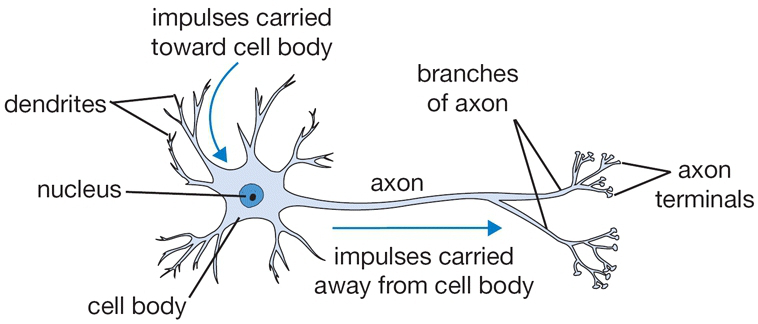
\includegraphics[width=0.6\columnwidth]{images/chap2/neuron.png}
    \footcaption{Cấu tạo một neural thần kinh}
    \label{chap2:animal_neural}
    \end{figure}
\end{center}
\footnotetext{Source: \url{http://cs231n.github.io/neural-networks-1/}}

\begin{center}
    \begin{figure}[H]
    \centering
    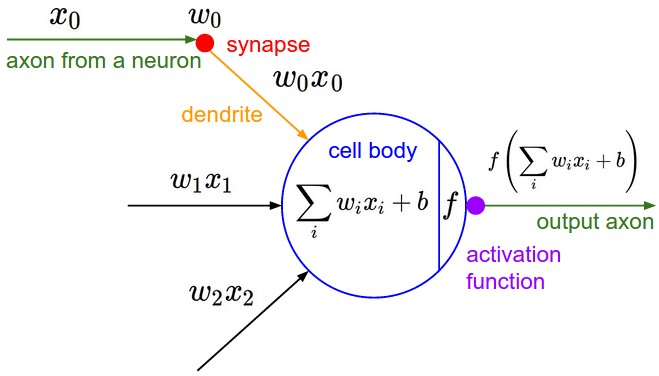
\includegraphics[width=0.6\columnwidth]{images/chap2/neuron_model.jpeg}
    \footcaption{Một mô hình neural dựa trên neural thần kinh}
    \label{chap2:neural_model}
    \end{figure}
\end{center}
\footnotetext{Source: \url{http://cs231n.github.io/neural-networks-1/}}


\subsection{Cấu tạo của neural}
Dựa trên cảm hứng về cấu tạo và hoạt động của mạng nơ-ron sinh học các nhà khoa học đã xây dựng ANN có cấu trúc và cách hoạt động tương tự với mong muốn xây dựng một mô hình mô phỏng lại những khả năng mạnh mẽ của bộ não người và áp dụng vào trong nhiều lĩnh vực khác nhau. Xét về cấu tạo ANN là một mạng lưới nhiều nơ-ron nhân tạo kết nối với nhau, ứng với mỗi cách kết nối ANN sẽ có đặc điểm và khả năng riệng biệt phù hợp với một loại ứng dụng nhất định.

\begin{figure}[H]
  \centering
  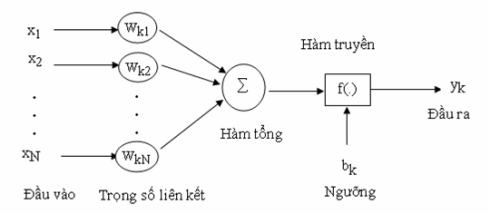
\includegraphics[width=0.9\textwidth]{images/chap2/norolnhantao.png}
  \footcaption{Cấu trúc một neural}
  \label{chap2:neural_structure}    
\end{figure}
\footnotetext{Nguồn: \url{https://tiendv.wordpress.com/2016/11/19/neural-networks/}}
Dựa vào hình \ref{chap2:neural_structure}, ta nhận thấy các thành phần cơ bản của một neural bao gồm:
\begin{description}
    \item[Các giá trị đầu vào] Dữ liệu này thường được đưa vào dưới dạng một vector N chiều
    \item[Các trọng số liên kết] Mỗi giá trị đầu vào được liên kết bởi một trọng số. Trọng số giữa đầu vào thứ j với neural k thường được kí hiện là $\displaystyle w_{kj}$. Các trọng số này lúc đầu sẽ được khởi tạo ngẫu nhiên, sau đó sẽ được cập nhật liên tục trong quá trình học.
    \item[Hàm tổng] Dùng để tính tổng các tích của các giá trị đầu vào với trọng số liên kết của nó.\\
    \begin{center}
        $\displaystyle u_k$ $=$ $\displaystyle \sum_{i=1}^nw_{ki}x_i$
    \end{center}{}
    \item[Ngưỡng] Còn gọi là Bias, là một thành phần của hàm truyền.
    \item[Hàm truyền] Còn gọi là Hàm kích hoạt (activation function), hàm này được dùng để giới hạn đầu ra của neural. Đầu vào của nó là tổng của Hàm tổng và Ngưỡng. Có rất nhiều hàm kích hoạt mà ta sẽ nói đến sau.
     \item[Đầu ra] Là giá trị đầu ra của neural, mỗi neural có nhiều nhất một giá trị đầu ra.
    \begin{center}
       %$\displaystyle y_k = f$$\displaystyle (z_k),$ với\\
       %$\displaystyle z_k = $ $\displaystyle \sum_{i=1}^nw_{ki}x_i + b_k\\
    \end{center}
\end{description}

Một số hàm kích hoạt thông dụng:
\begin{figure}[H]
  \centering
  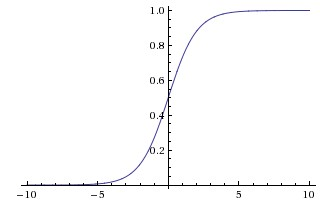
\includegraphics[width=0.5\textwidth]{images/chap2/sigmoid.jpeg}
  \footcaption{Hàm Sigmoid giới hạn đầu ra trong khoảng (0, 1)} 
  \label{chap2:fig08}    
\end{figure}
\footnotetext{Source: \url{http://brohrer.github.io/how_convolutional_neural_networks_work.html}} 

\begin{figure}[H]
  \centering
  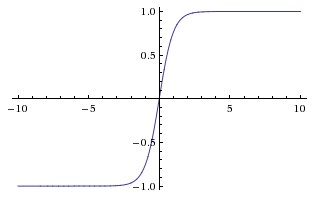
\includegraphics[width=0.5\textwidth]{images/chap2/tanh.jpeg}
  \footcaption{Hàm Tanh giới hạn đầu ra trong khoảng (-1, 1)} 
  \label{chap2:fig08}    
\end{figure}
\footnotetext{Source: \url{http://brohrer.github.io/how_convolutional_neural_networks_work.html}} 

\begin{figure}[H]
  \centering
  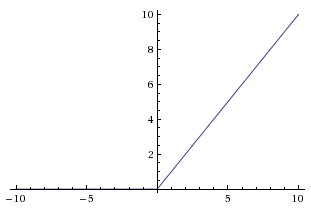
\includegraphics[width=0.5\textwidth]{images/chap2/relu.jpeg}
  \footcaption{Hàm ReLU, bằng 0 khi x < 0 và thuộc đường thẳng có hệ số góc là 1 khi x > 0} 
  \label{chap2:fig08}    
\end{figure}
\footnotetext{Source: \url{http://brohrer.github.io/how_convolutional_neural_networks_work.html}} 

Với các bài toán binary đơn giản, dữ liệu là khả tách tuyến tính, tức là tồn tại một đường thẳng có thể phân chia tập dữ liệu ra làm hai, khả năng biểu diễn của một neural đơn lẻ tỏ ra hiệu quả, tức có thể tìm được một đường thẳng giúp phân chia hai lớp của hàm. Tuy nhiên, trường hợp dữ liệu không khả tách tuyến tính, chúng ta cần kết hợp nhiều neural với nhau tạo thành một mạng neural để có thể giải quyết bài toán phân lớp phi tuyến.


Hình \ref{chap2:neural_logic} mô tả một vài hàm logic đơn giản có thể được biểu diễn dưới một neural và trường hợp phép toán XOR, trường hợp phân lớp phi tuyến, không tìm được lời giải chỉ với một neural.
\begin{center}
    \begin{figure}[H]
    \centering
    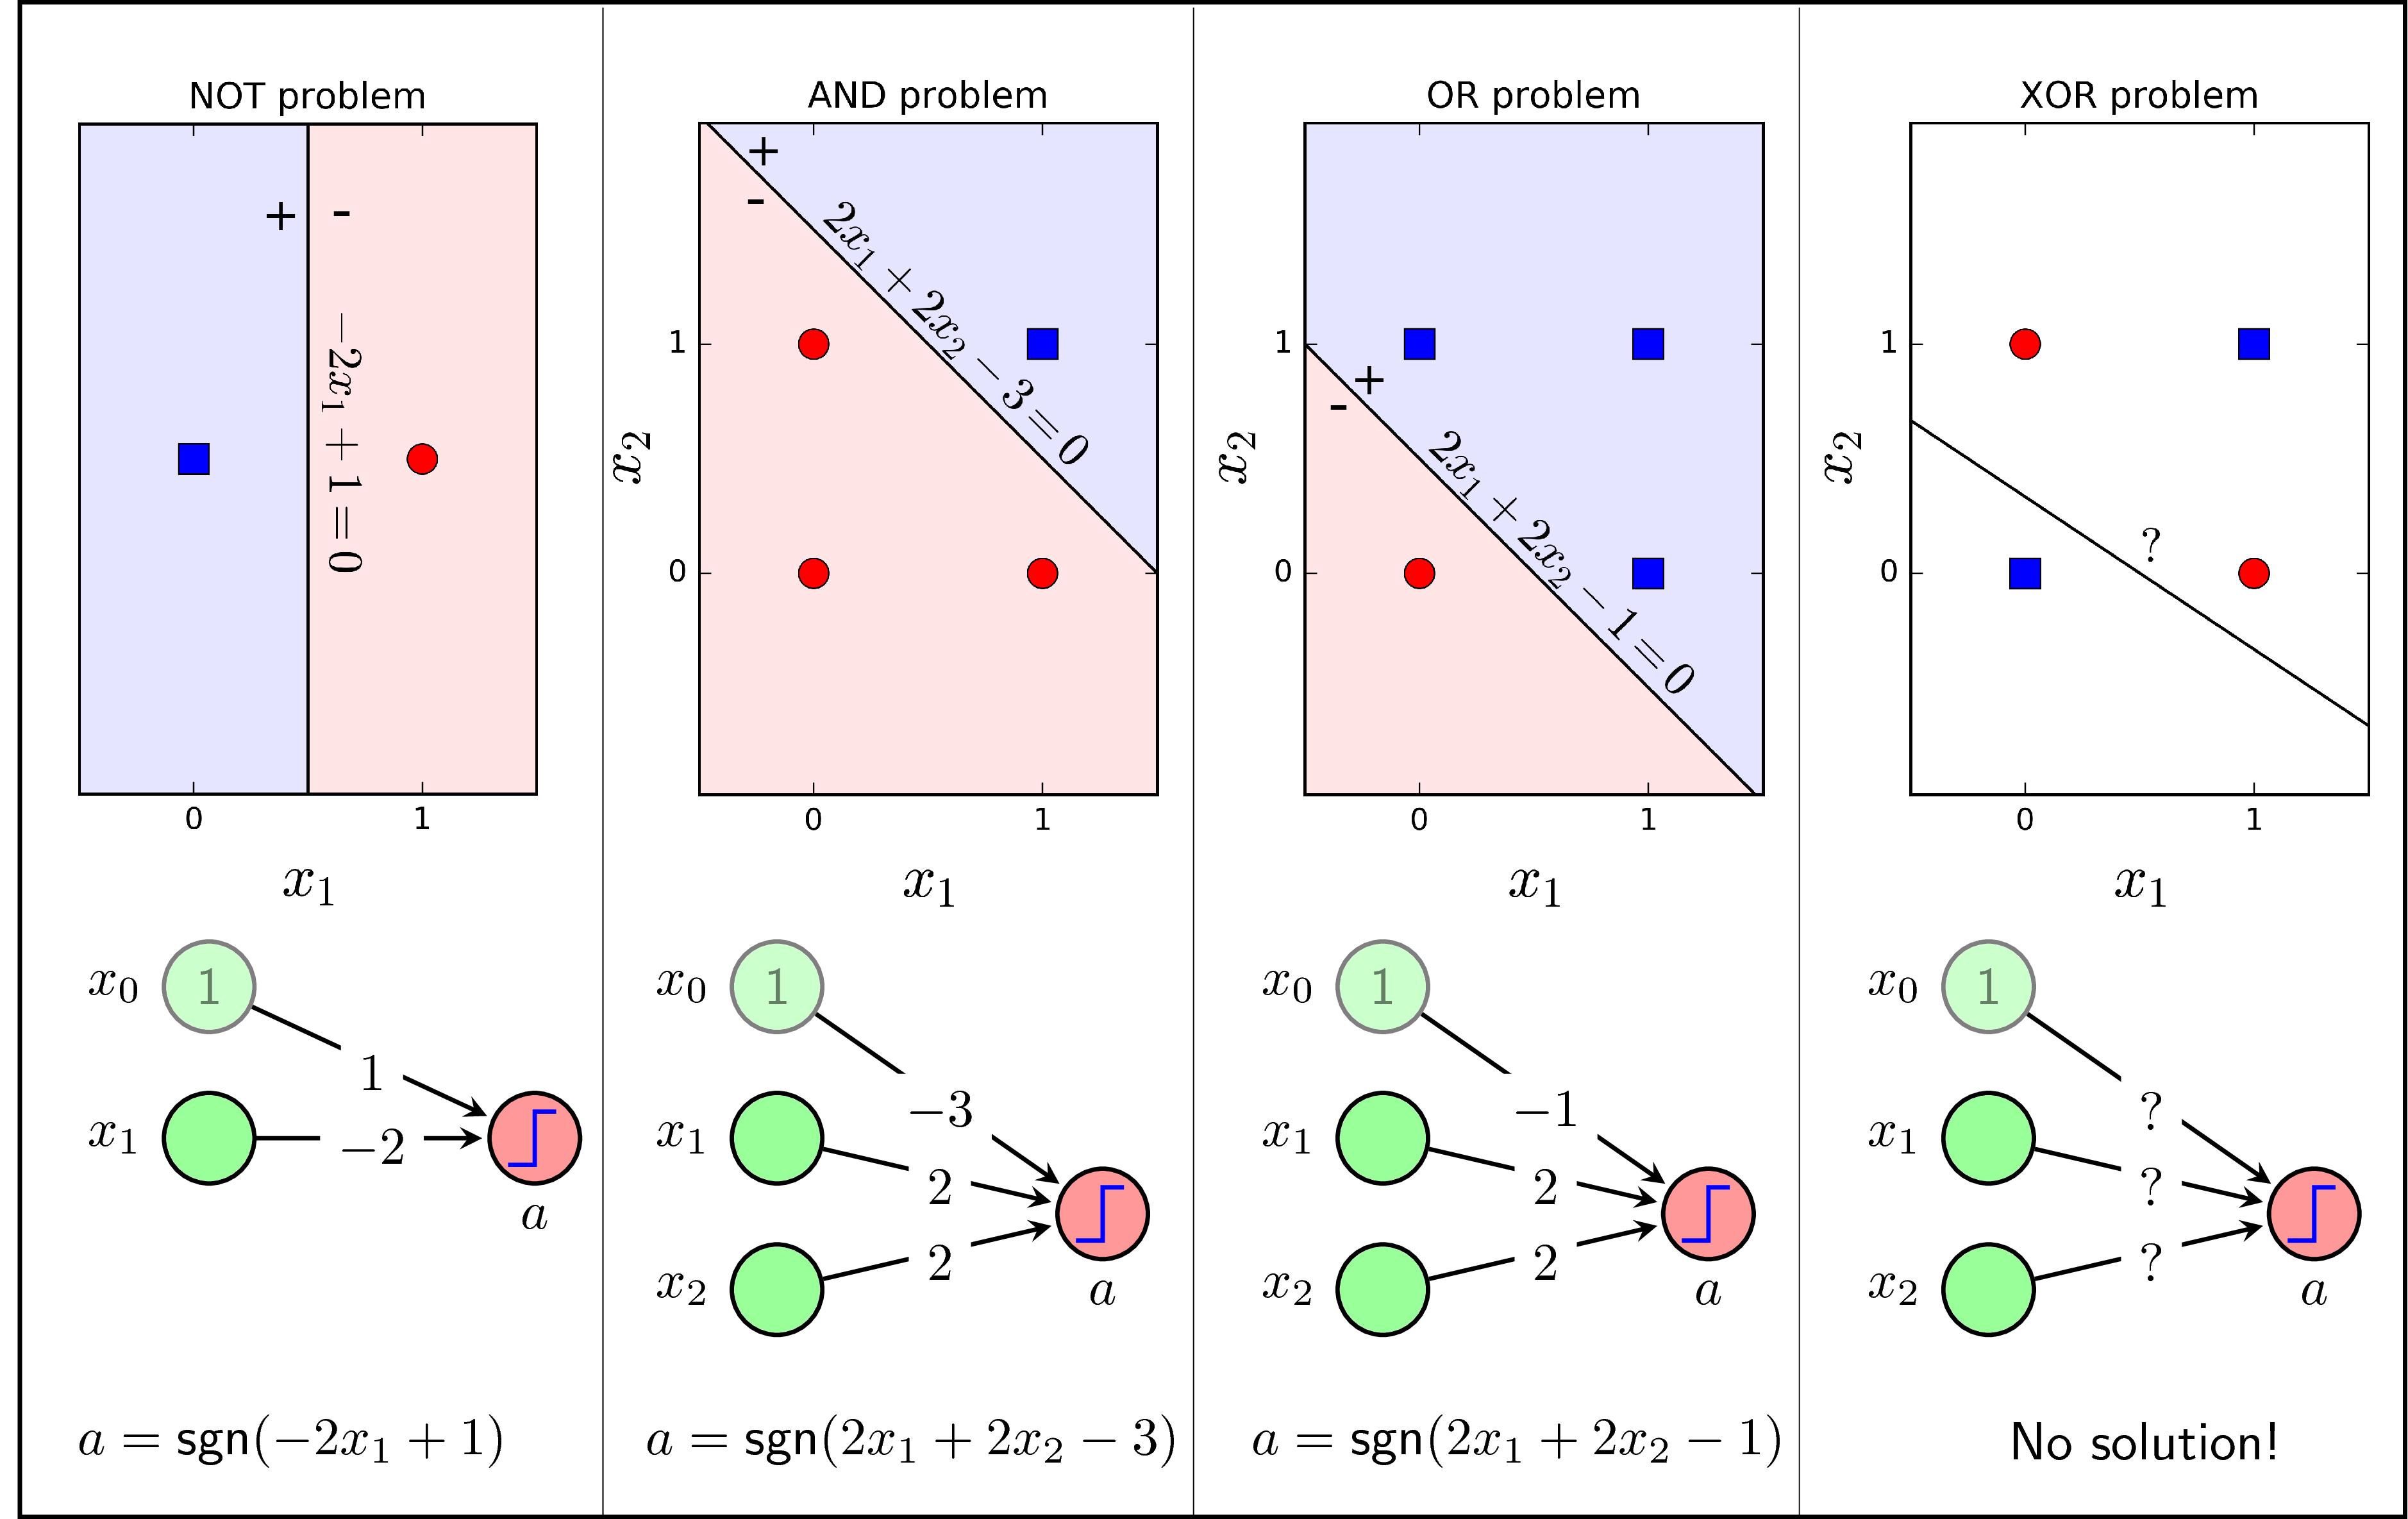
\includegraphics[width=1\columnwidth]{images/chap2/logic_nn.png}
    \footcaption{Mạng neural với một neural có thể biểu diễn được các hàm logic đơn giản}
    \label{chap2:neural_logic}
    \end{figure}
\end{center}
\footnotetext{Source: \url{https://machinelearningcoban.com/2017/02/24/mlp/}}

\subsection{ Cấu trúc mạng neural}
Nhiều neural kết hợp lại tạo thành mạng neural. Tùy vào cách kết nối mà ANN tạo nên kiến trúc riêng của nó. Có thể hiểu rằng các neural kết nối với nhau bằng cách một hoặc một vài đầu ra của neural này có thể là đầu vào của neural khác.

ANN thường được cấu trúc từ các lớp (layer) riêng biệt, các lớp thường là lớp kết nối đầy đủ (fully-connected layer - FC) hoặc lớp kết nối một phần (spartially-connected layer), nhưng phổ biến hơn cả vẫn là các lớp kết nối đầy đủ.

\begin{center}
    \begin{figure}[H]
    \centering
    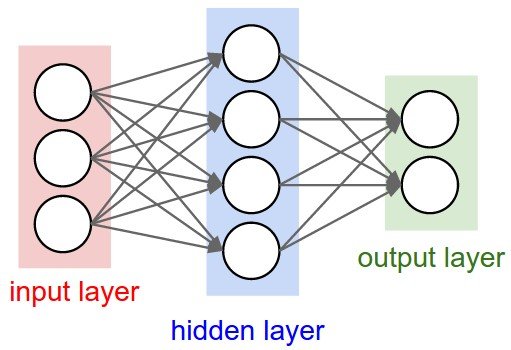
\includegraphics[width=0.5\columnwidth]{images/chap2/2layer.jpeg}
    \footcaption{Mạng neural hai lớp đầy đủ, với một lớp đầu vào 3 neural, lớp ẩn 4 neural và lớp đầu ra 2 neural. Các neural ở lớp khác nhau kết nối với nhau và không kết nối với các neural trong cùng lớp}
    \label{fig:my_label}
    \end{figure}
\end{center}
\footnotetext{Source: \url{http://cs231n.github.io/neural-networks-1/}}
\begin{center}
    \begin{figure}[H]
    \centering
    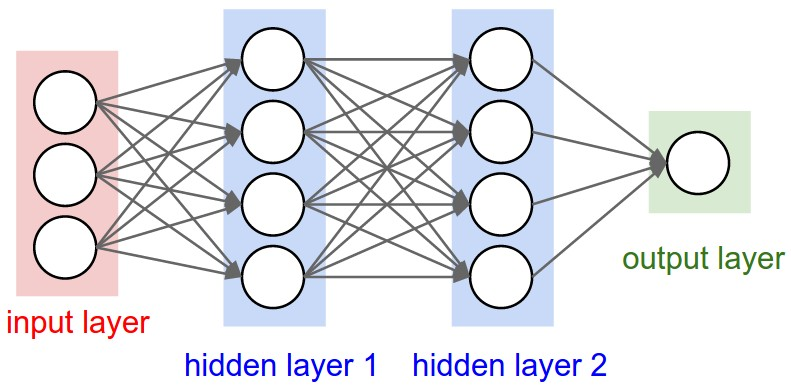
\includegraphics[width=0.6\columnwidth]{images/chap2/3layer.jpeg}
    \footcaption{Mạng neural ba lớp đầy đủ với hai lớp ẩn, mỗi lớp 4 neural}
    \label{fig:my_label}
    \end{figure}
\end{center}
\footnotetext{Source: \url{http://cs231n.github.io/neural-networks-1/}}


\begin{center}
    \begin{figure}[H]
    \centering
    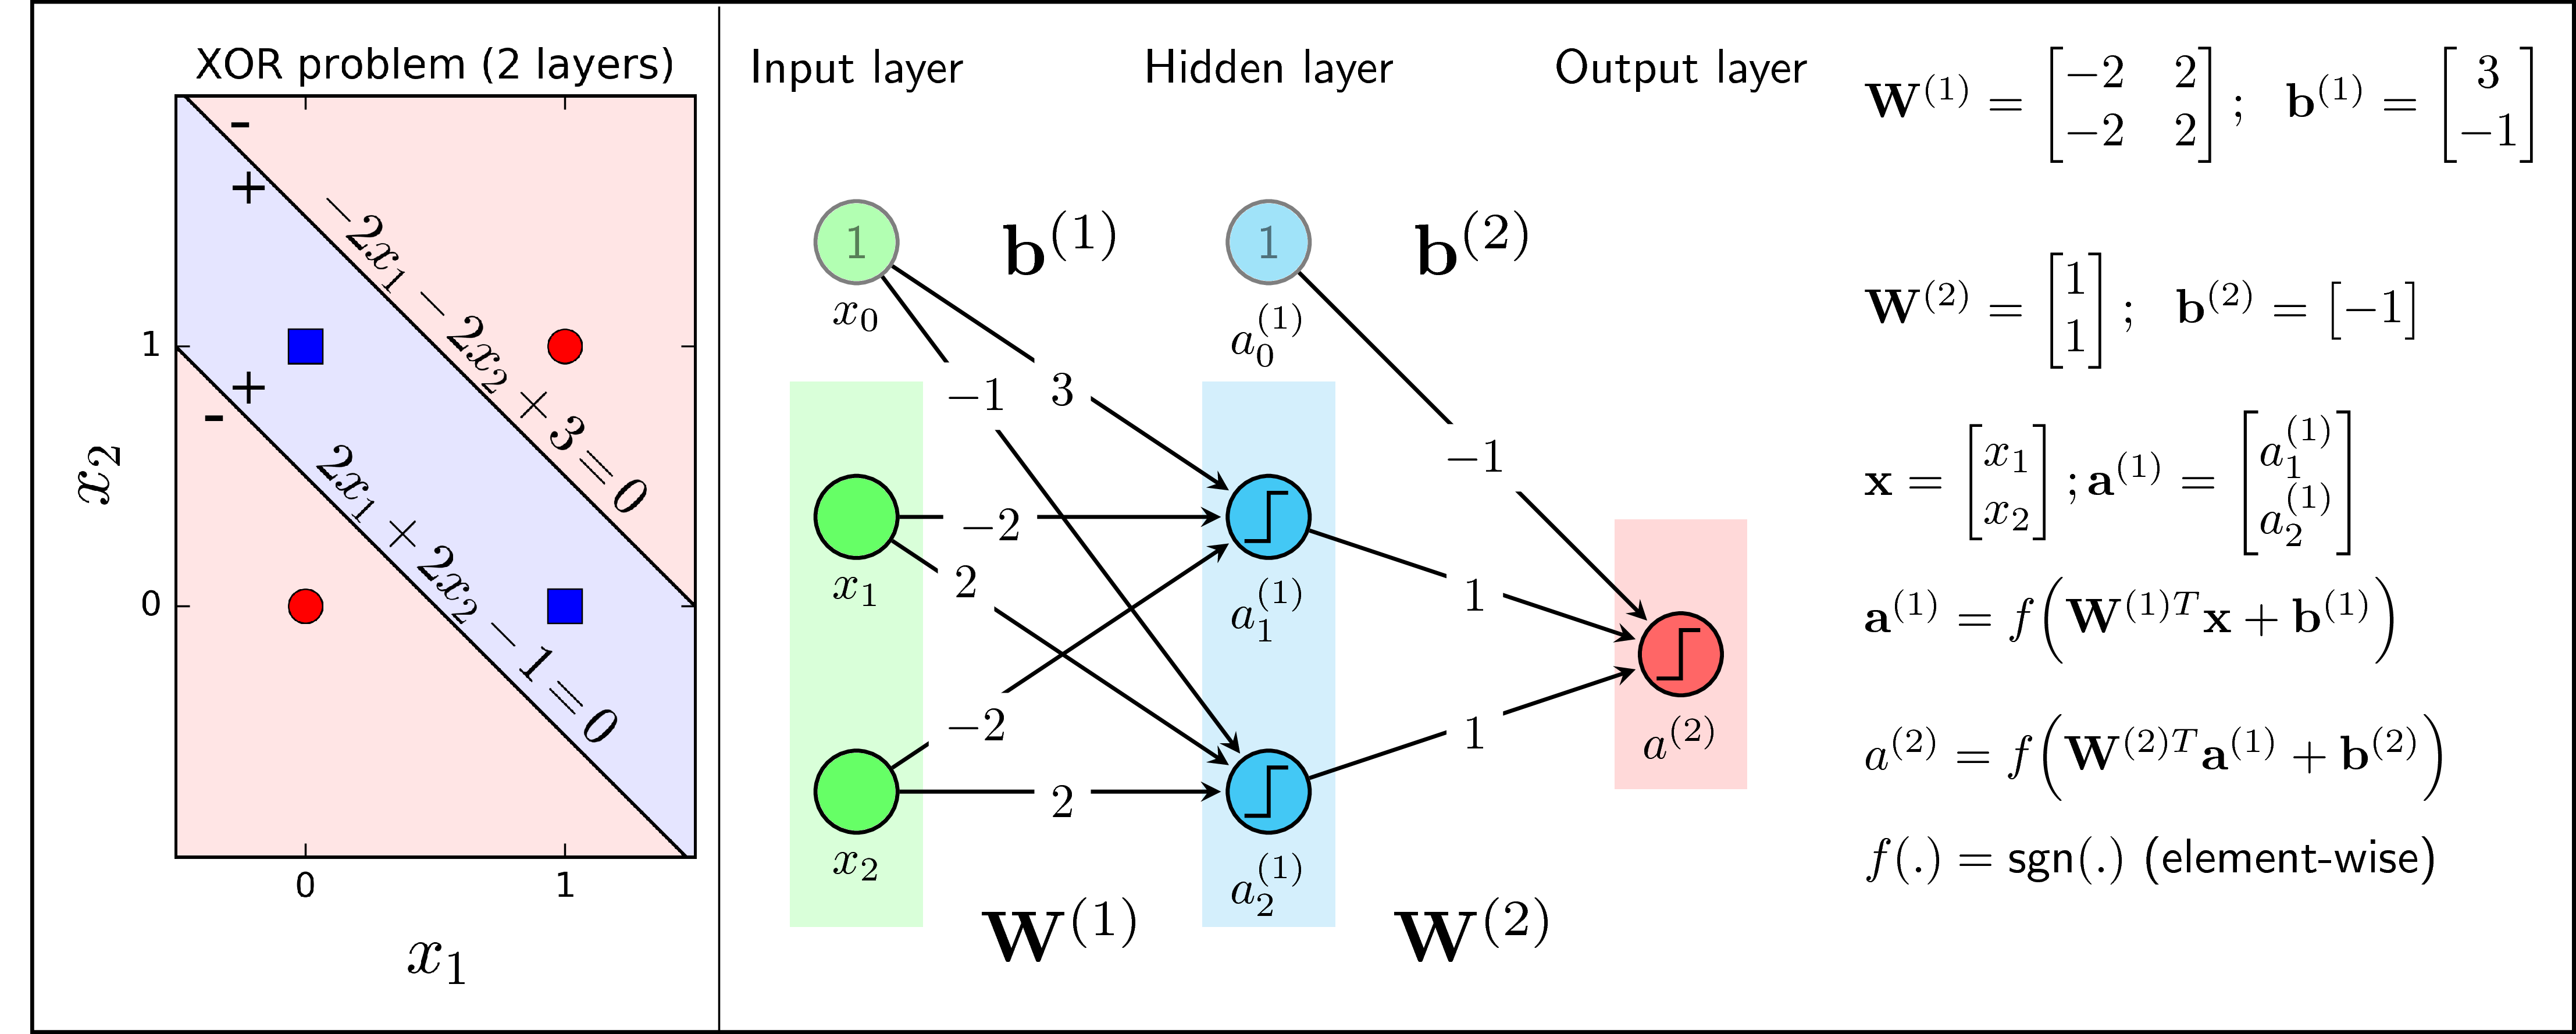
\includegraphics[width=1\columnwidth]{images/chap2/xor_nn.png}
    \footcaption{Mạng neural biểu diễn hàm XOR}
    \label{fig:my_label}
    \end{figure}
\end{center}
\footnotetext{Source: \url{https://machinelearningcoban.com/2017/02/24/mlp/}}
Mạng neural trở nên hiệu quả hơn với các dữ liệu phân bố phi tuyến. Tuy vậy, lựa chọn số lớp ẩn là một vấn đề không hề đơn giản. Về cơ bản, số lớp tăng cũng như kích thước mạng tăng, các neural sẽ biểu diễn được nhiều hàm phức tạp hơn, nhưng từ đó cũng dễ dẫn đến overfit hơn. 

\begin{center}
    \begin{figure}[H]
    \centering
    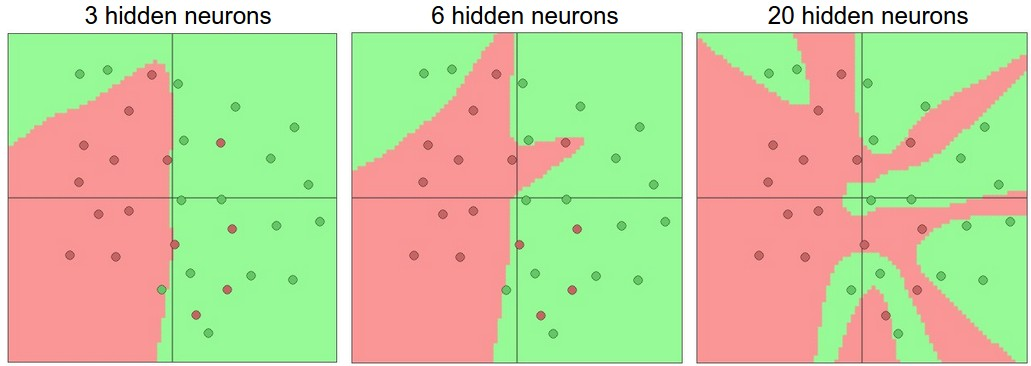
\includegraphics[width=1\columnwidth]{images/chap2/layer_sizes.jpeg}
    \footcaption{Ba mạng neural khác nhau cho cùng một tập dữ liệu, sau khi được huấn luyện cho ra ba kết quả khác nhau}
    \label{chap2:three_net}
    \end{figure}
\end{center}
\footnotetext{Source: \url{http://cs231n.github.io/neural-networks-1/}}

Ta có thể thấy từ hình \ref{chap2:three_net}, mô hình 3 lớp ẩn không hoàn toàn tổng quát hóa được các lớp của dữ liệu. Trong khi đó, mô hình 20 lớp ẩn bị overfit do nó phân lớp cả những điểm nhiễu. Nhưng đừng vì vậy mà chọn mô hình nhỏ hơn chỉ vì nó không bị overfit.

Trong thực tế, người ta không chọn những mô hình nhỏ hơn để tránh overfit, vì những mô hình này không hiệu quả với các thuật toán huấn luyện local như Gradient Descent (GD), thay vào đó, họ vẫn chọn mô hình lớn nhất phần cứng có thể hỗ trợ được, sau đó kết hợp các kĩ thuật xử lí, giảm thiểu nhiễu và overfit để đạt được kết quả khả quan hơn.

\subsection{Hàm mất mát}
Hàm mất mát, kí hiệu là \textbf{L}, là một thành phần của \textbf{\(L_D\)}. Trong công thức:
\begin{center}
	\begin{equation}
		L_D(f_w) = \frac{1}{\lvert D \rvert}\sum_{(x, y)\in D}L(f_w(x), y)
	\end{equation}
\end{center}
\textbf{\(L_D\)} là tổng của trung bình cộng các \textbf{L}. Hàm mất mát trả về một số thực không âm thể hiện sự chênh lệch giữa hai đại lượng \textbf{\^{y}}- label được dự đoán, và \textbf{y} - label đúng. Hàm này có tác dụng để đo sự sai lệch giữa giá trị dự đoán và giá trị được gán nhãn ban đầu, tức giá trị của hàm càng nhỏ thì độ sai sót càng ít, kết quả dự đoán được càng gần với kết quả mong muốn. Trong trường hợp lý tưởng, tức là khi \textbf{\^{y}} \textbf{ = y}, hàm mất mát đạt giá trị cực tiểu bằng 0.

Ta nhận thấy hàm mất mát của một mô hình phải thỏa mãn các tiêu chí sau:
\begin{itemize}
	\item Hàm mất mát phải liên tục, khả vi, vì các phương pháp thông dụng để cực tiểu hóa hàm mất mát thường đòi hỏi phải tính được đạo hàm
	\item Khi model dự đoán sai, ta cần phải phạt model nhiều hơn khi model dự đoán gần đúng, tức là hàm mất mát sẽ lớn hơn khi model dự đoán một kết quả xa hơn kết quả mong đợi.
\end{itemize}

Một số hàm mất mát cơ bản:
\begin{itemize}
	\item Hàm \textbf{Square Loss}
	\begin{center}
		\begin{equation}
			L(\hat{y}, y) = \frac{1}{2}(\hat{y} - y)^2
		\end{equation}
	\end{center}
	Hàm này thường được dùng cho cả mục đích classification và regression, nhưng vẫn được dùng trong regression nhiều hơn.
	\item Hàm \textbf{0-1 Loss}
	Hàm này trả về 1 nếu \textbf{\^{y}}.\textbf{y} < 0, và trả về 0 nếu ngược lại. Hàm này không có đạo hàm ở điểm 0 nên thường được dùng để tính error rate của mô hình chứ không dùng để huấn luyện mô hình.
	\item Hàm \textbf{Perceptron Loss}
	\begin{center}
		\begin{equation}
			L_{perceptron}(\hat{y}, y) = max(0, \hat{y}.y)
		\end{equation}
	\end{center}
	Đối với \textbf{Perceptron Loss}, mô hình dành cho các bài toán Binary Classification, một trong các đặc điểm là khi mô hình đoán đúng thì \textbf{\^{y}} cùng dấu với \textbf{y}, \textbf{\^{y}}.\textbf{y} < 0. Khi đó:
	\begin{center}
		\begin{equation}
			L_{perceptron}(\hat{y}, y) = max(0, <0) = 0
		\end{equation}
	\end{center}
	Từ đó ta thấy, hàm mất mát này không phân biệt giữa các dự đoán đúng, nhưng lại phạt những dự đoán sai.
	\item Hàm \textbf{Hinge Loss}
	\begin{center}
		\begin{equation}
			L_{hinge}(\hat{y}, y) = max(0, 1-\hat{y}.y)
		\end{equation}
	\end{center}
	Dễ dàng thấy \textbf{Hinge Loss} chính là một biến thể của \textbf{Perceptron Loss}, chỉ là thêm 1 đơn vị vào -\textbf{\^{y}}.\textbf{y}, số 1 này được gọi là \textbf{margin}. Hàm này cho kết quả gần tương tự như \textbf{Perceptron Loss}, chỉ trừ các dự đoán mà \textbf{\^{y}}.\textbf{y} nằm trong khoảng [0, 1]. Kết quả rơi vào khoảng này toàn là kết quả đúng, nhưng \textbf{Hinge Loss} muốn phân biệt các kết quả đúng với nhau, nhưng khi \textbf{\^{y}}.\textbf{y} vượt quá 1 thì hàm không phân biệt nữa. Bởi vì khi nằm trong khoảng [0, 1], kết quả đưa ra là những dự đoán gần ranh giới.
	
Ý tưởng của \textbf{Hinge Loss} là muốn khuyến khích mô hình đưa ra những quyết định có tính chắc chắn cao, nằm ngoài ranh giới để không bị phạt nữa.
	\item Hàm \textbf{Logistic Loss}
	\begin{center}
		\begin{equation}
			L(\hat{y}, y) = log_2(1 + exp(-\hat{y}.y))
		\end{equation}
	\end{center}
	Đây là một hàm liên tục, không âm và không tăng. Một điểm khác biệt giữa \textbf{Logistic Loss} với hai hàm mất mát ở trên là đồ thị của nó có một độ cong nhất định, tức là nó không giảm với tốc độ như nhau ở mọi điểm. Trong khi một phần của \textbf{Perceptron Loss} và \textbf{Hinge Loss} là một đường tuyến tính có tốc độ như nhau tại mọi điểm.
	
	Việc chọn hàm mất mát nào phụ thuộc rất lớn vào tính chất bài toán, ứng dụng và đặc biệt là dữ liệu có sẵn. Hình \ref{chap2:loss_function} dưới đây là đồ thị trực quan từng hàm mất mát.
	\begin{center}
    \begin{figure}[H]
    \centering
    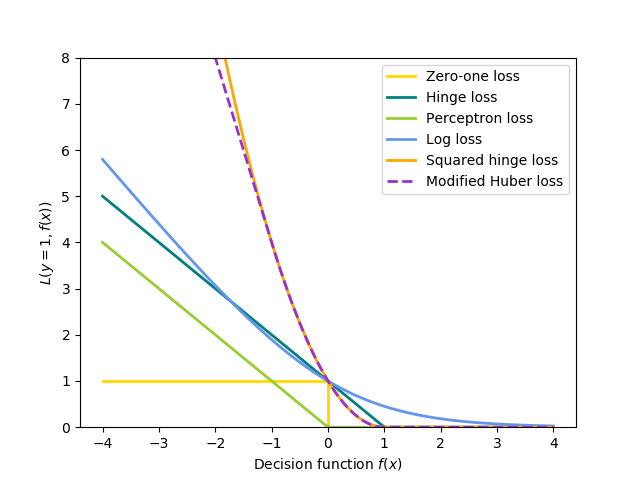
\includegraphics[width=0.7\columnwidth]{images/chap2/loss_plot.png}
    \caption{Đồ thị các hàm mất mát}
    \label{chap2:loss_function}
    \end{figure}
\end{center}
\end{itemize}

\subsection{Giải thuật lan truyền ngược (Backpropagation)}
Có thể hiểu mạng neural nhân tạo là một mạng nhận vào một tập các dữ liệu huấn luyện \textbf{X}, sau quá trình huấn luyện sẽ cho ra một tập weight \textbf{W} và bias \textbf{b}. Hàm \textbf{f(W, b, x)}  với x là input của bài toán, chính là mô hình thu được bằng mạng neural nhân tạo. Mạng càng chính xác thì \textbf{f(W, b, x)} càng cho kết quả gần với thực tế.

Có nhiều phương pháp để tối ưu \textbf{W}, nhưng phổ biến nhất vẫn là sử dụng \textbf{Gradient Descent} (GD). Để áp dụng GD, ta cần tính hàm mất mát của mô hình theo W và b. Giả sử \textbf{J(W, b, x)} là một hàm mất mát, để áp dụng GD, ta phải tính được:
\begin{center}
	\begin{equation}
		\frac{\partial J}{\partial W};
		\frac{\partial J}{\partial b}
	\end{equation}
\end{center}
Ví dụ hàm mất mát là hàm Square Loss, ta có:
\begin{center}
	\begin{equation}
		J(W, b, x) = \frac{1}{N}\sum_{n=1}^N||y_n - \hat{y}_n||^2_2
	\end{equation}
\end{center}
Với N là số mẫu trong tập training.

Theo công thức ở trên, hàm mất mát không phụ thuộc trực tiếp vào W và b, nên việc tính đạo hàm \(\frac{\partial J}{\partial W}\) và \(\frac{\partial J}{\partial b}\) là rất phức tạp. Do vậy, thuật toán Backpropagation thường được sử dụng cùng với gradient để tính ngược từ lớp cuối cùng về lớp đầu tiên nhằm tìm lượng thay đổi \(\Delta W\) hay \(\Delta b\) tương ứng giúp tối ưu hóa W và b.

Lớp cuối cùng được tính đầu tiên vì nó gần với lớp ouput và hàm mất mát nhất. Đạo hàm các lớp trước được tính theo quy tắc \textit{chain rule}, tức đạo hàm của hàm hợp.

Ví dụ, đạo hàm của hàm mất mát của trọng số ở lớp cuối cùng:
\begin{center}
	\begin{equation}
		\frac{\partial J}{\partial w_{ij}^{(L)}} = \frac{\partial J}{\partial z_j^{(L)}}.\frac{\partial z_j^{(L)}}{\partial w_{ij}^{(L)}} 
		= e_j^{(L)}a_i^{(L-1)}
	\end{equation}
\end{center}
Trong đó \(\frac{\partial z_j^{(L)}}{\partial w_{ij}^{(L)}} = a_i^{(L-1)}\) vì \(z_j^{(L)} = w_j^{(L)}a^{(L-1)}+b_j^{(L)}\)
Tương tự, đạo hàm của hàm mất mát theo b ở lớp cuối cùng:
\begin{center}
	\begin{equation}
		\frac{\partial J}{\partial b_{j}^{(L)}} = \frac{\partial J}{\partial z_j^{(L)}}.\frac{\partial z_j^{(L)}}{\partial b_{j}^{(L)}} 
		= e_j^{(L)}
	\end{equation}
\end{center}
Hình \ref{chap2:backpropagation} dưới đây mô tả trực quan cách tính Backpropagation qua các biến số và các lớp của mạng:
\begin{center}
    \begin{figure}[H]
    \centering
    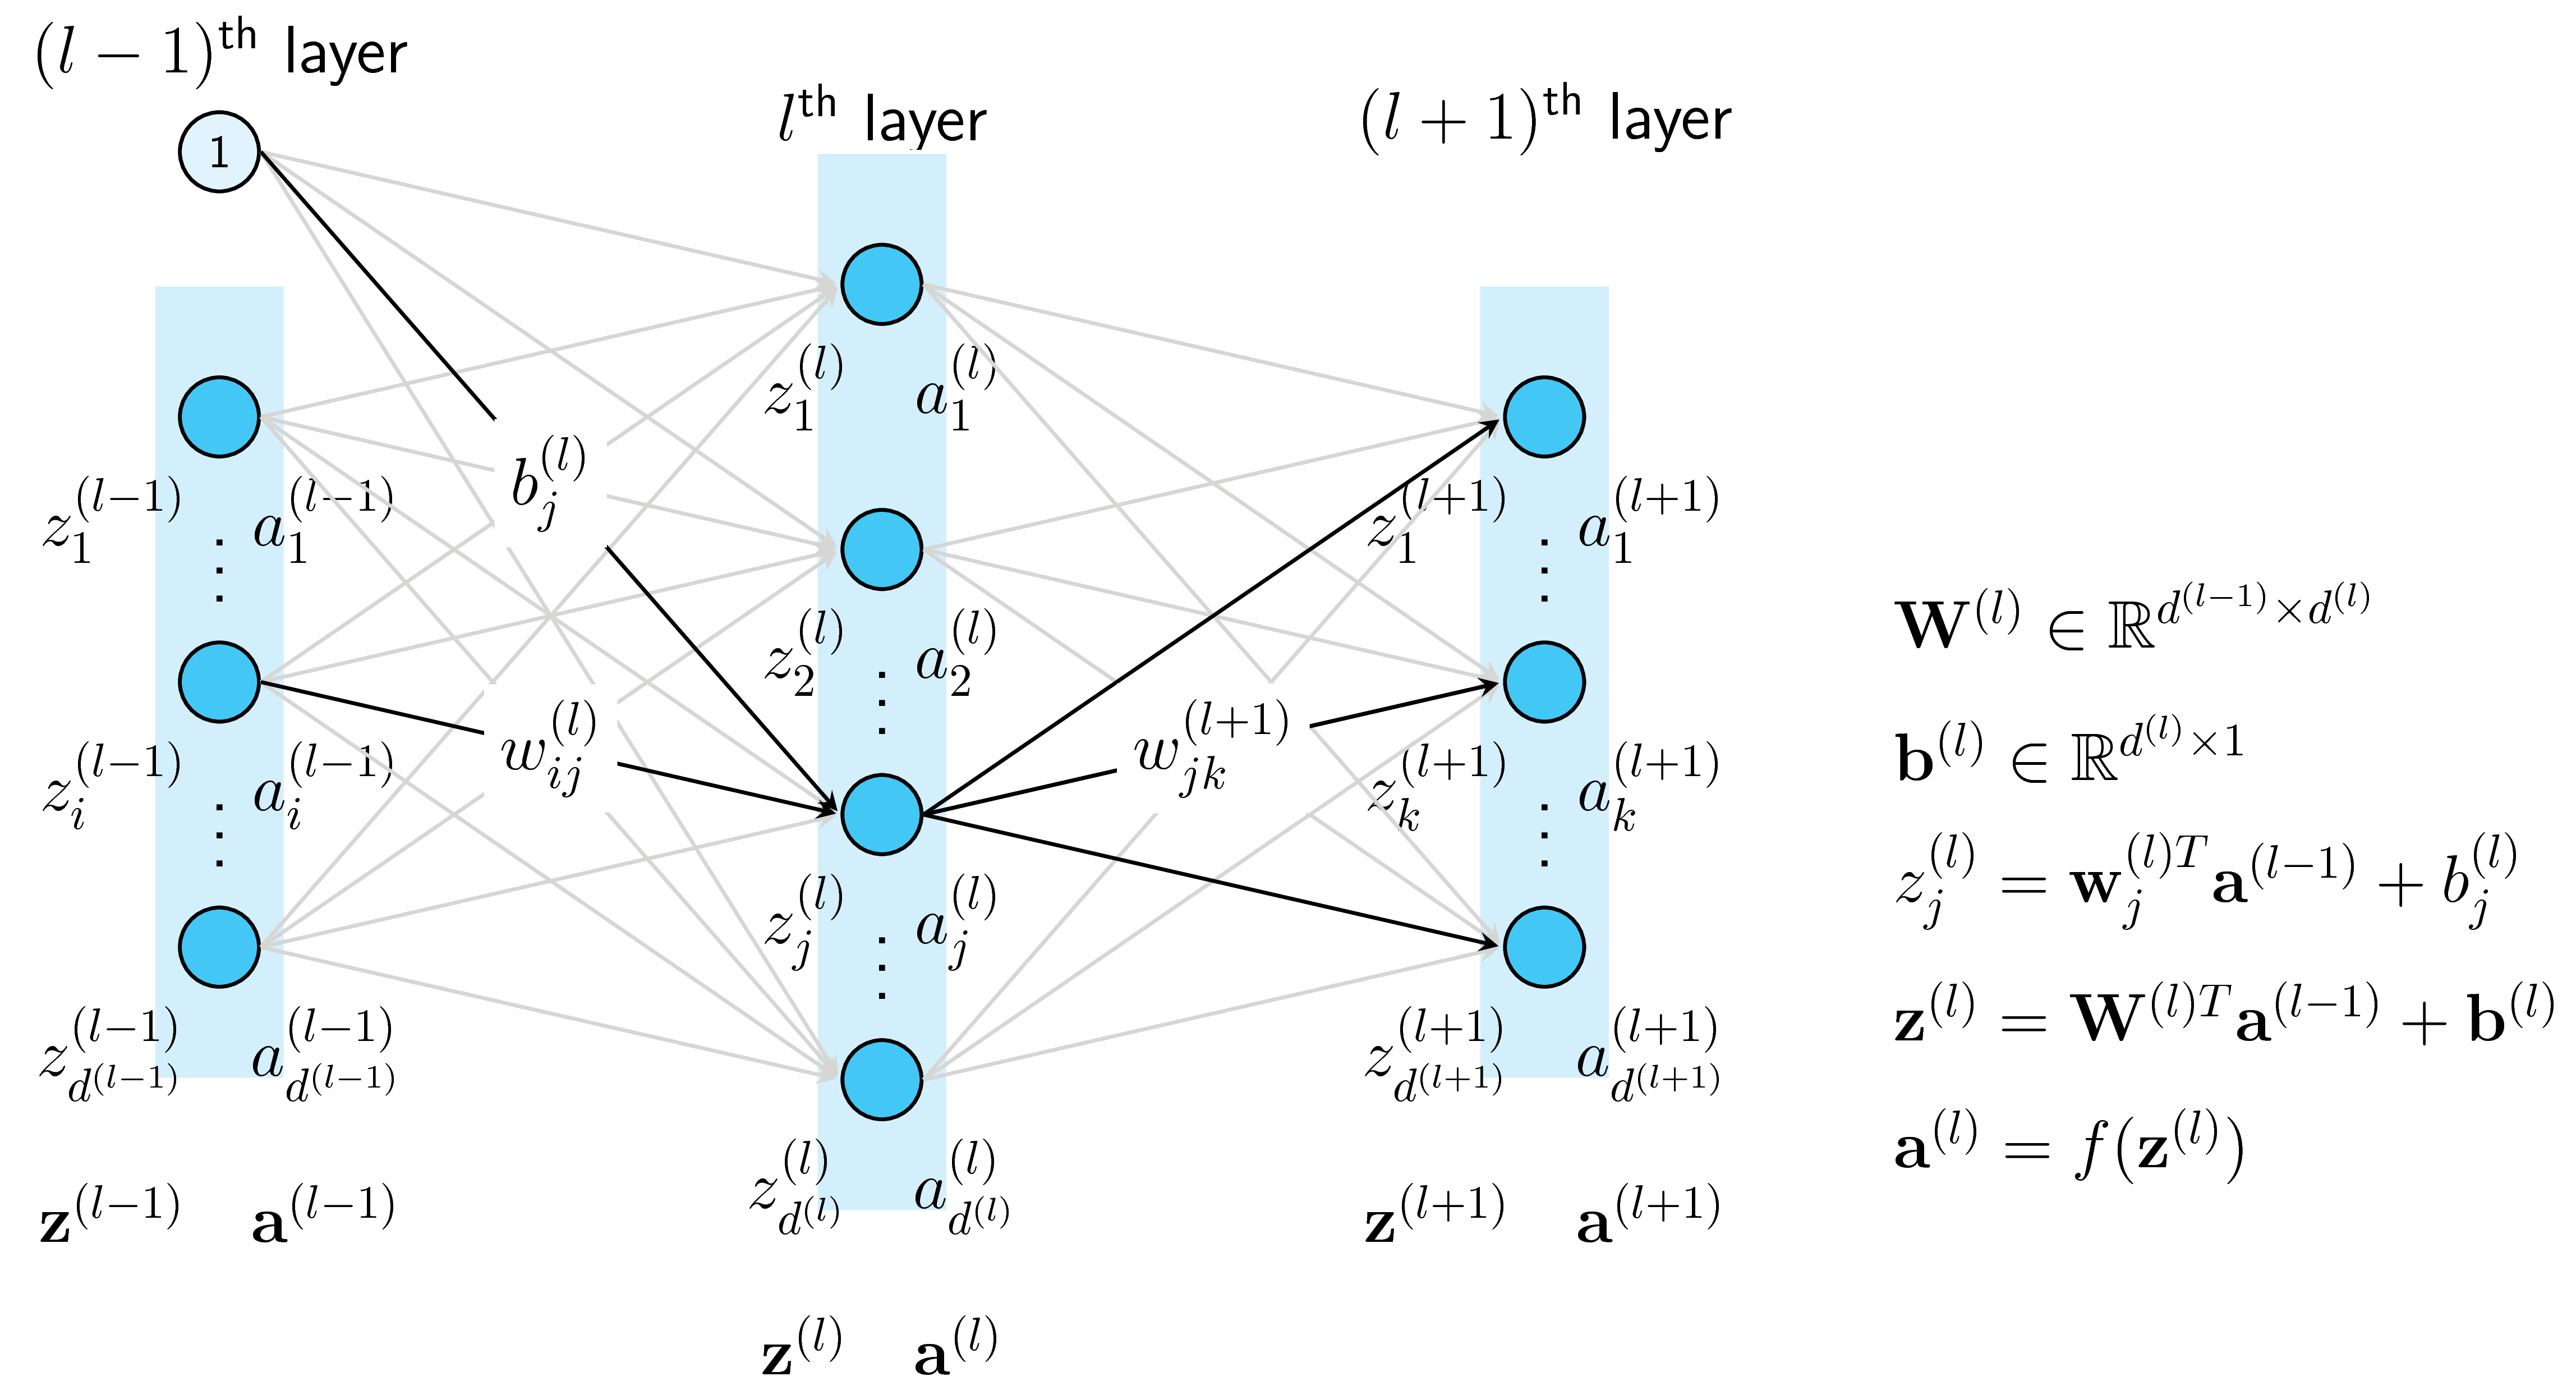
\includegraphics[width=1\columnwidth]{images/chap2/backpropagation.png}
    \footcaption{Cách tính Backpropagation}
    \label{chap2:backpropagation}
    \end{figure}
\end{center}
\footnotetext{Source: \url{https://machinelearningcoban.com/2017/02/24/mlp/}}
Từ hình trên ta có:
\begin{center}
	\begin{equation}
		\frac{\partial J}{\partial w_{ij}^{(l)}} = \frac{\partial J}{\partial z_j^{(l)}}.\frac{\partial z_j^{(l)}}{\partial w_{ij}^{(l)}} 
		= e_j^{(l)}a_i^{(l-1)}
	\end{equation}
\end{center}
trong đó:
\begin{align}
		e_j^{(l)} & = \frac{\partial J}{\partial z_j^{(l)}} = \frac{\partial J}{\partial a_j^{(l)}}.\frac{\partial a_j^{(l)}}{\partial z_j^{(l)}} \nonumber\\
		& = (\sum_{k=1}^{d^{(l+1)}} \frac{\partial J}{\partial z_k^{(l+1)}}.\frac{\partial z_k^{(l+1)}}{\partial a_j^{(l)}} )f'(z_j^{(l)}) \nonumber\\
		& = (\sum_{k=1}^{d^{(l+1)}} e_k^{(l+1)}w_{jk}^{(l+1)} )f'(z_j^{(l)}) \nonumber\\
		& = (e^{(l+1)}w_{j:}^{(l+1)})f'(z_j^{(l)}) \nonumber\\
\end{align}
Tương tự ta có hàm mất mát so với b trên từng lớp của mạng:
	\begin{align}
	\frac{\partial J}{\partial b_j^{(l)}} = e_j^{(l)}
\end{align}
Với \( (e_j^{(l+1)} = [e_1^{(l+1)}, e_2^{(l+1)},...,e_{d^{(l+1)}}^{(l+1)}])^T \)

Từ các công thức trên, ta thấy việc tính \(e_j^{(l)}\) rất quan trọng. Muốn tính \(e_j^{(l)}\) ta phải tính được \(e_j^{(l+1)}\), tức tính ngược giá trị này từ cuối. Đó là nguồn gốc cho tên Backpropagation của giải thuật này.

\section{Mạng neural tích chập}
\subsection{Định nghĩa}
Mạng neural nhân tạo ra đời đã được ứng dụng và thành công trong nhiều bài toán phân loại và nhận dạng. Tuy nhiên, ANN không thực sự hiệu quả đối với những dữ liệu có dạng hình ảnh. Chính sự liên kết quá đầy đủ đã tạo nên những khó khăn cho mô hình vì dữ liệu hình ảnh có kích thước khá lớn. Chính vì lẽ đó Mạng neural tích chập ra đời, với ý tưởng thay vì toàn bộ ảnh kết nối với một node, nay một node chỉ cần kết nối với một phần của ảnh, từ đó dữ liệu hình ảnh thông qua các lớp của mô hình này sẽ được huấn luyện thành các đặc điểm (feature) và tiến hành phân lớp.

CNN là một trong những mô hình Deep Learning hiện nay giúp chúng ta giải quyết các vấn đề về thị giác máy tính như nhận diện, phân loại ảnh với độ chính xác cao. Về cơ bản, CNN là một mạng ANN truyền thẳng và bao gồm các lớp sau: lớp \textbf{Convolutional}, lớp \textbf{ReLU}, lớp \textbf{Pooling} và lớp  \textbf{Fully connected}. Số lượng và thứ tự giữa các lớp này sẽ tạo ra những mô hình khác nhau phù hợp cho từng bài toán khác nhau.


Hình \ref{chap2:cnn_example} mô tả cấu trúc một mạng neural tích chập từ input, qua các lớp Convolution, Pooling, Fully Connected đến output.
\begin{center}
    \begin{figure}[H]
    \centering
    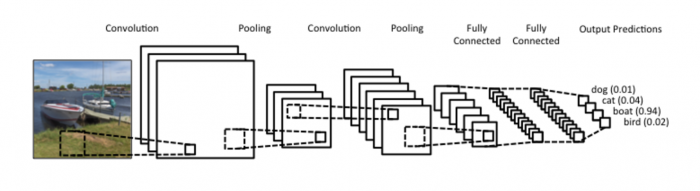
\includegraphics[width=1\columnwidth]{images/chap2/cnn.png}
    \footcaption{Một mạng neural tích chập}
    \label{chap2:cnn_example}
    \end{figure}
\end{center}
\footnotetext{Source: \url{http://www.wildml.com/2015/11/understanding-convolutional-neural-networks-for-nlp/}}

\subsection{Lớp Convolutional}
Lớp Convolutional là lớp quan trọng nhất trong mô hình CNN. Lớp này ra đời dựa trên cơ sở lý thuyết tín hiệu số, việc tính tích chập sẽ giúp trích xuất được những thông tin quan trọng từ hình ảnh. Phép tính này được thực hiện bằng cách trượt một cửa sổ mà ta gọi là sliding window (hoặc kernel, filter hay feature detector) trên ma trận hình ảnh đầu vào, trong đó kết quả phép toán mỗi lần trượt được tính như Hình \ref{chap2:calculation}, với sliding window có kích thước 2x2, trên toàn bộ ma trận kích thước 3x4.

\begin{center}
    \begin{figure}[H]
    \centering
    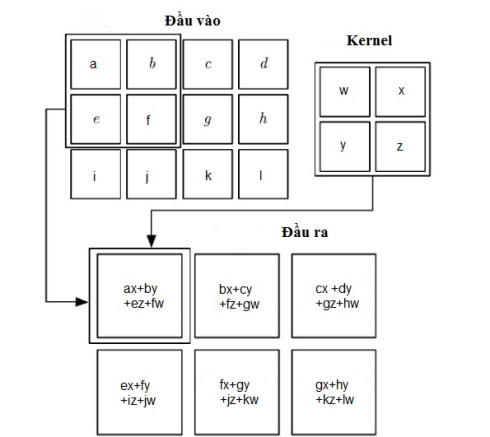
\includegraphics[width=0.6\columnwidth]{images/chap2/viduveconvulution.jpg}
    \caption{Ví dụ về phép tính tích chập}
    \label{chap2:calculation}
    \end{figure}
\end{center}

Số phần tử trong ma trận đầu ra cũng là số ảnh sẽ truyền vào lớp tiếp theo. Trong quá trình huấn luyện, các trọng số của các filder ban đầu sẽ được khởi tạo ngẫu nhiên, sau đó sẽ được cập nhật liên tục.

Sau khi áp dụng các tính toán, ta nhận thấy rằng các thông tin hình ảnh ban đầu đã được biến đổi thành các feature (cạnh, hướng, hình dạng, màu sắc,...). Hình \ref{chap2:result_filter} minh họa việc áp dụng phép tính tích chập lên một ảnh có sẵn.

\begin{center}
    \begin{figure}[H]
    \centering
    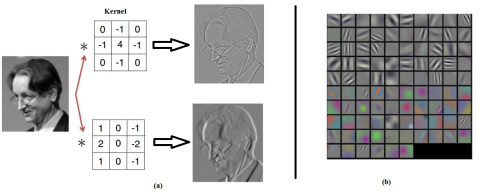
\includegraphics[width=0.8\columnwidth]{images/chap2/viduapplyconvu.jpg}
    \footcaption{(a) Kết quả biến đổi hình ảnh khi thực hiện với các filter khác nhau (b) Các feature được trích xuất từ hình ảnh gốc}
    \label{chap2:result_filter}
    \end{figure}
\end{center}
\footnotetext{Source: \url{http://cs231n.stanford.edu/}}


Đóng vai trò tuy nhỏ nhưng quan trọng trong quá trình này là lớp ReLU (Rectified Linear Unit). Do lớp trước (convolutional) là một phép biến đổi tuyến tính, nên tại mỗi neural cần có một hàm kích hoạt dưới dạng phi tuyến. Có nhiều hàm kích hoạt được sử dụng nhưng các nghiên cứu gần đây cho thấy ReLU có nhiều ưu điểm vượt trội hơn cả, điển hình là cài đặt nhanh và tính toán đơn giản hơn rất nhiều.

Lớp ReLU thường được cài đặt ngay sau lớp Convolutional. Hàm kích hoạt của nó là $f(x) = max(0, x)$, nói một cách trực quan thì lớp này chuyển các giá trị âm từ lớp Convolutional thành 0, nhằm tạo tính phi tuyến cho mô hình (hình \ref{chap2:relu}).
\begin{center}
    \begin{figure}[H]
    \centering
    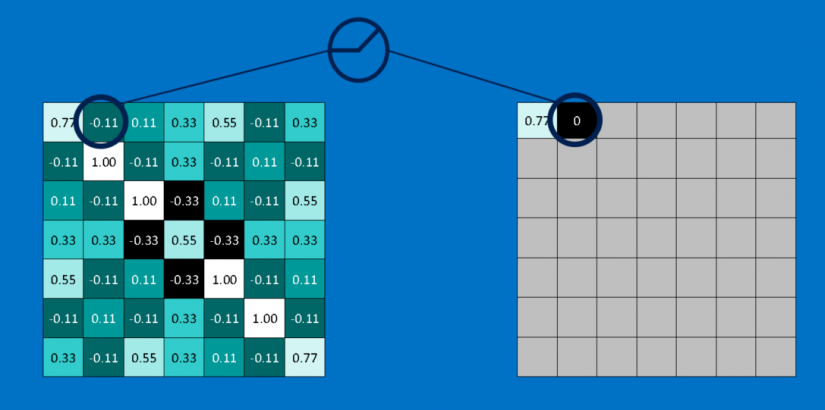
\includegraphics[width=0.8\columnwidth]{images/chap2/relu_array.png}
    \footcaption{Output của layer ReLU giống với output của layer Convolutional, chỉ khác ở chỗ loại bỏ các giá trị âm }
    \label{chap2:relu}
    \end{figure}
\end{center}
\footnotetext{Source: \url{https://brohrer.github.io/how_convolutional_neural_networks_work.html}}

\subsection{Lớp Pooling}
Pooling là một trong những thành phần chính và mạnh mẽ của CNNs. Pooling thực chất là quá trình tính toán trên ma trận để đạt được kết quả là một ma trận nhỏ hơn nhưng vẫn giữ nguyên những feature của ma trận gốc. Pooling tính toán rất đơn giản, với mỗi bước filter trượt trên ảnh gốc, nó sẽ chọn giá trị lớn nhất trong filter đó ở mỗi bước. Như vậy đầu ra sẽ có cùng số lượng hình ảnh nhưng số điểm ảnh lại giảm đáng kể. Ví dụ, giảm số điểm ảnh của một tấm ảnh xuống 4 lần sẽ giúp mọi xử lý trở nên dễ dàng, nhanh chóng.

Một ảnh sau khi qua lớp Pooling vừa được thu nhỏ, vừa bảo toàn tính khớp với mỗi feature. Do đó CNNs vẫn có thể tìm xem liệu một feature có nằm trong hình ảnh hay không, từ đó vẫn cho kết quả chính xác.

\begin{center}
    \begin{figure}[H]
    \centering
    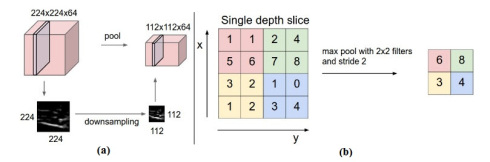
\includegraphics[width=0.8\columnwidth]{images/chap2/pool.jpg}
    \footcaption{Tính toán trên lớp Pooling}
    \label{fig:my_label}
    \end{figure}
\end{center}
\footnotetext{Source: \url{http://cs231n.github.io/convolutional-networks/}}

\begin{center}
    \begin{figure}[H]
    \centering
    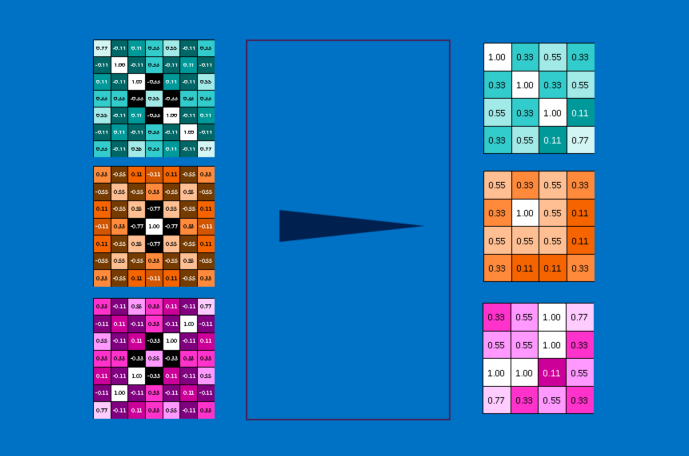
\includegraphics[width=0.6\columnwidth]{images/chap2/resize.png}
    \footcaption{Đầu ra có cùng số lượng ảnh nhưng kích thước bị giảm, tuy vậy vẫn giữ nguyên các feature trước đó}
    \label{fig:my_label}
    \end{figure}
\end{center}
\footnotetext{Source: \url{https://brohrer.github.io/how_convolutional_neural_networks_work.html}}

\subsection{Lớp Fully-connected}
Fully-connected tương tự với lớp trong ANN. Các giá trị ở lớp trước được liên kết đầy đủ vào các node của lớp tiếp theo. Trong CNN, lớp này thường xuất hiện ở các tầng cuối của mô hình. Vì ảnh đã được xử lý và trích xuất feature từ các lớp trước nên dữ liệu sẽ không còn quá lớn, ta dễ dàng sử dụng FC để tiến hành nhận dạng thông qua các vote.

\begin{center}
    \begin{figure}[H]
    \centering
    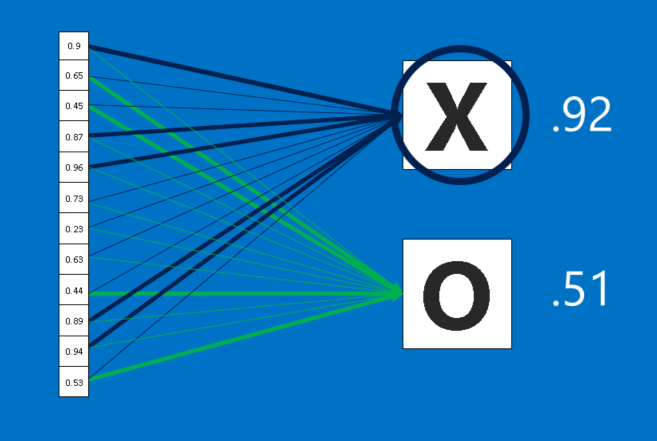
\includegraphics[width=0.5\columnwidth]{images/chap2/fc_vote.png}
    \footcaption{Lớp FC lấy hình ảnh ở các lớp trước rồi chuyển thành các vote (trong hình là phân loại X và O)}
    \label{fig:my_label}
    \end{figure}
\end{center}
\footnotetext{Source: \url{https://brohrer.github.io/how_convolutional_neural_networks_work.html}}

\section{Thuật toán nhận diện hình ảnh}
Có rất nhiều phương pháp nhận diện hình ảnh (Hình \ref{chap2:object_detection_example}), trong đó Faster R-CNN là một trong những phương pháp hiện đại và hiệu quả cho tới ngày nay. Đó là phương pháp phân loại vật thể và xác định vị trí của vật thể đó trong ảnh, trong đó cho output là tọa độ của một hình chữ nhật, đồng thời xác định vật thể bên trong hình chữ nhật đó là gì. Faster R-CNN đã trải qua nhiều phiên bản, trong đó không thể không nhắc tới R-CNN và Fast R-CNN.

\begin{center}
    \begin{figure}[H]
    \centering
    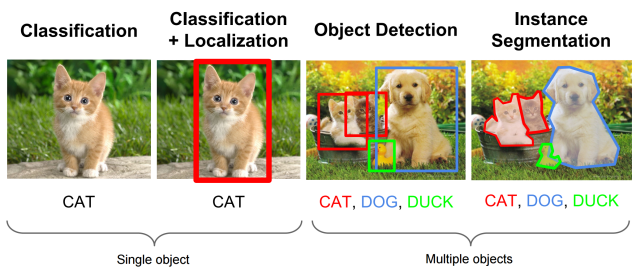
\includegraphics[width=0.6\columnwidth]{images/chap2/LocalizationDetection.png}
    \footcaption{Mô tả bài toán tìm kiếm vị trí vật thể trong ảnh}
    \label{chap2:object_detection_example}
    \end{figure}
\end{center}
\footnotetext{Nguồn: \url{http://cs231n.stanford.edu/slides/2016/winter1516_lecture8.pdf}}
\subsection{Localization bằng phương pháp hồi quy}
Hồi quy có thể được dùng làm phương pháp để xác định được tọa độ của bounding box trong bài toán học có giám sát. Bounding box là khung hình chữ nhật để xác định tọa độ của vật thể trong hình. Trong quá trình huấn luyện mạng nơ-ron, tọa độ này thường được dự đoán ra dưới dạng gồm 4 số ($x_0$, $y_0$, chiều dài, chiều rộng). Kết quả này sẽ được so sánh với tọa độ bounding box của vật đã được gán nhãn. Hàm lỗi khoảng cách Euclidean sẽ được áp dụng để tính lỗi và cập nhật lại trọng số cho mô hình mạng huấn luyện (Hình \ref{fig:2.22}).
\begin{center}
    \begin{figure}[H]
    \centering
    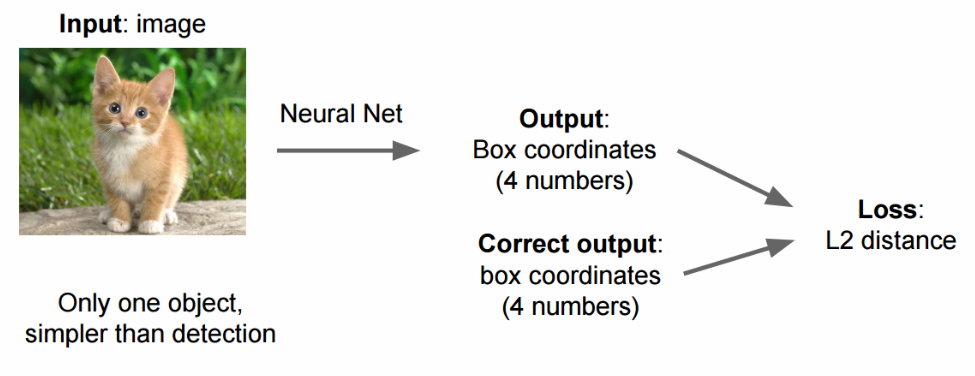
\includegraphics[width=0.8\columnwidth]{images/chap2/localization_1.png}
    \footcaption{Localization bằng phương pháp hồi quy cho mạng nơ-ron}
    \label{fig:2.22}
    \end{figure}
\end{center}
\footnotetext{Nguồn: \url{http://cs231n.stanford.edu/slides/2016/winter1516_lecture8.pdf}}
Cách đơn giản để thực hiện phân loại và localization, gồm có 4 bước:\\
\begin{enumerate}
	\item Huấn luyện một mô hình phân loại hoặc sử dụng mô hình phân loại đã có sẵn (AlexNet, VGG, GoogLeNet)
	\begin{center}
    \begin{figure}[H]
    \centering
    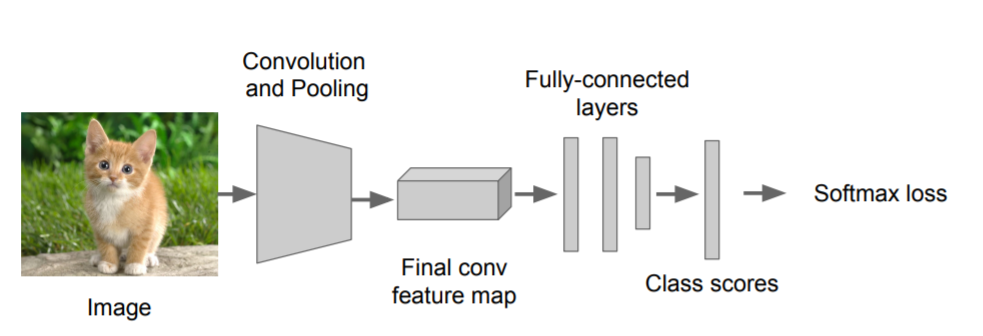
\includegraphics[width=0.8\columnwidth]{images/chap2/localization_2.png}
    \footcaption{Localization bằng phương pháp hồi quy cho mạng nơ-ron - bước 1}
    \label{fig:2.23}
    \end{figure}
	\end{center}
	\footnotetext{Nguồn: \url{http://cs231n.stanford.edu/slides/2016/winter1516_lecture8.pdf}}
	Những mô hình này thường dùng các lớp mạng tích chập và lớp pooling để trích xuất ra feature map (bản đồ đặc trưng), từ đó đưa qua một hoặc nhiều lớp fully-connected để tính được điểm phân loại (Hình \ref{fig:2.23}).
	\item  Thêm các đầu hồi quy vào sau các lớp fully-connected để xác định bounding box
	\begin{center}
    \begin{figure}[H]
    \centering
    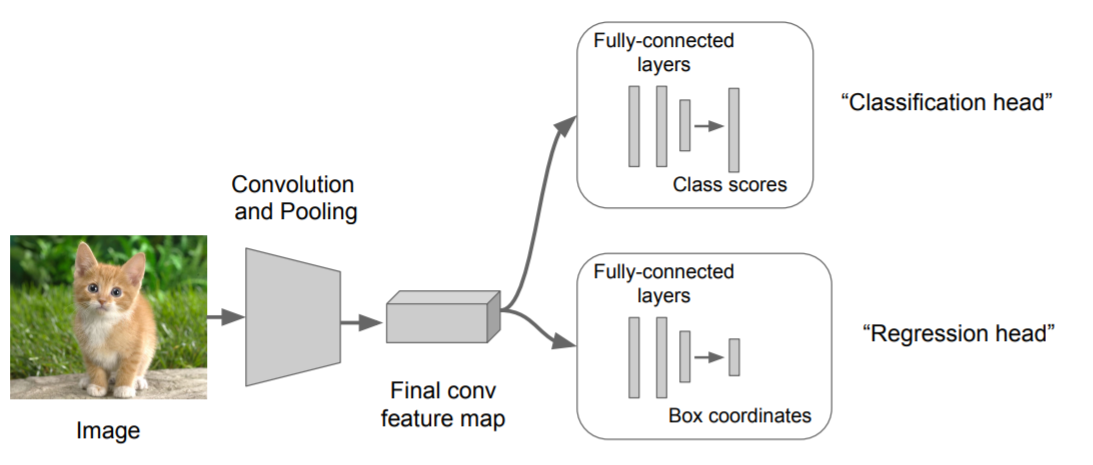
\includegraphics[width=0.8\columnwidth]{images/chap2/localization_3.png}
    \footcaption{Localization bằng phương pháp hồi quy cho mạng nơ-ron - bước 2}
    \label{fig:2.24}
    \end{figure}
	\end{center}
	\footnotetext{Nguồn: \url{http://cs231n.stanford.edu/slides/2016/winter1516_lecture8.pdf}}
	Ở bước này, mô hình mạng được mở thêm một nhánh từ feature map. Nhánh này cũng đi qua một hoặc nhiều lớp fully-connected nhưng nó không dùng để tính điểm phân loại nữa mà sẽ áp dụng phương pháp hồi quy để tính ra tọa độ của bounding box (Hình \ref{fig:2.24}).
	\item Huấn luyện riêng đầu hồi quy với stochastic gradient descent và hàm lỗi L2 (Eclidean distance loss)
	\begin{center}
    \begin{figure}[H]
    \centering
    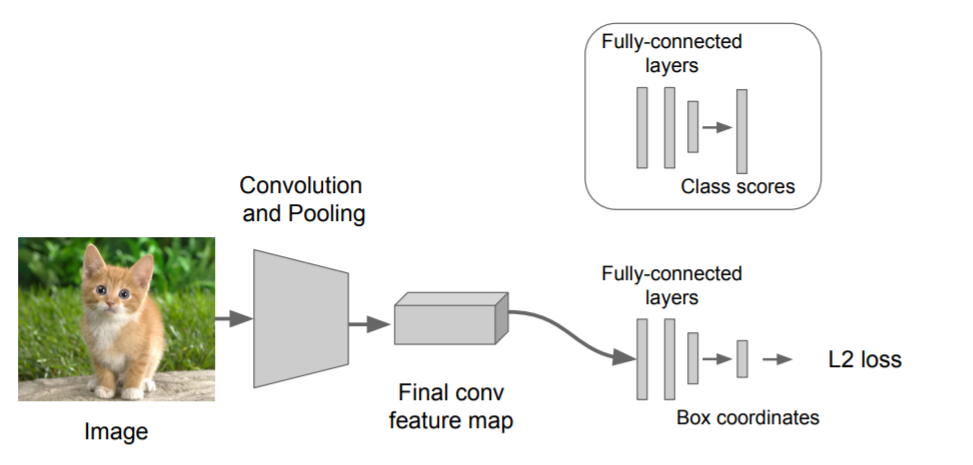
\includegraphics[width=0.8\columnwidth]{images/chap2/localization_4.png}
    \footcaption{Localization bằng phương pháp hồi quy cho mạng nơ-ron - bước 3}
    \label{fig:2.25}
    \end{figure}
	\end{center}
	\footnotetext{Nguồn: \url{http://cs231n.stanford.edu/slides/2016/winter1516_lecture8.pdf}}
	Kết quả dự đoán bounding box sẽ được so với ground-truth box (tọa độ vật thể được gán nhãn trước đó) từ đó tính hàm lỗi và cập nhật lại trọng số cho riêng nhánh mạng hồi quy bằng kĩ thuật stochastic gradient descent (Hình \ref{fig:2.25}).
	\item Dùng cả hai bộ phân loại và hồi quy lúc chạy kết quả
	\begin{center}
    \begin{figure}[H]
    \centering
    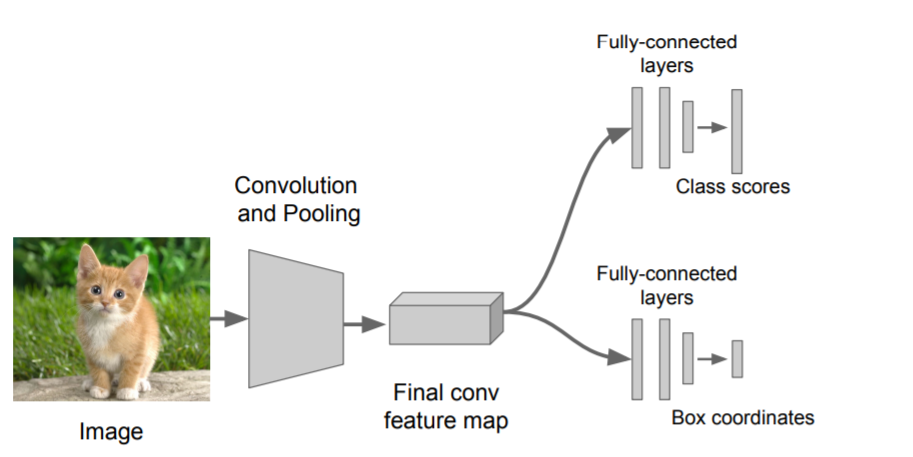
\includegraphics[width=0.8\columnwidth]{images/chap2/localization_5.png}
    \footcaption{Localization bằng phương pháp hồi quy cho mạng nơ-ron - bước 4}
    \label{fig:2.26}
    \end{figure}
	\end{center}
	\footnotetext{Nguồn: \url{http://cs231n.stanford.edu/slides/2016/winter1516_lecture8.pdf}}
	Hàm lỗi L2 được áp dụng để tính lỗi và cập nhật lại trọng số cho nhánh hồi quy dựa theo phương pháp stochastic gradient descent (Hình \ref{fig:2.26}).
\end{enumerate}
Sau khi huấn luyện xong, mô hình có thể sử dụng bằng cách đưa ảnh cần dự đoán vào và thực hiện phân loại cùng với hồi quy để xác định được vật thể thuộc nhãn nào và đánh dấu nó trên hình.
Tuy nhiên hạn chế của phương pháp này chính là chỉ có thể tìm được một vật thể ở mỗi lần hoạt động.
\subsection{Region based Convolutional Neural Network - R-CNN}
R-CNN (Regions + CNN) là một phương pháp nhận diện hình ảnh dựa vào một hệ thống sinh các bounding boxes (hay còn gọi là region proposals), chứa các vùng có khả năng bao gồm các vật thể ở trong.

\begin{center}
    \begin{figure}[H]
    \centering
    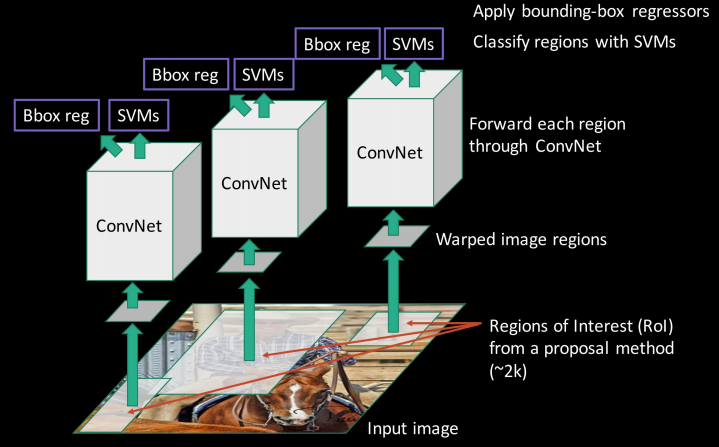
\includegraphics[width=0.6\columnwidth]{images/chap2/RCNNSimple.png}
    \footcaption{Mô hình R-CNN đơn giản}
    \label{fig:2.27}
    \end{figure}
\end{center}
\footnotetext{Nguồn: \url{http://cs231n.stanford.edu/slides/2016/winter1516_lecture8.pdf}}
Hình \ref{fig:2.27} mô tả kiến trúc của mô hình R-CNN, từ ảnh đầu vào ta sẽ tìm các RoI và đưa mỗi RoI qua CNN để trích xuất đặc trưng, cuối cùng dùng SVM và phương pháp hồi quy để phân loại và tìm ra bounding box của vật.
Khuyết điểm lớn nhất của R-CNN chính là thời gian hiện thực. Cụ thể, mô hình được huấn luyện theo các bước như sau:

\begin{enumerate}
    \item Dùng một mạng CNN đã được huấn luyện sẵn (như Alexnet hay VGG-16)
    \begin{center}
    	\begin{figure}[H]
	    \centering
	    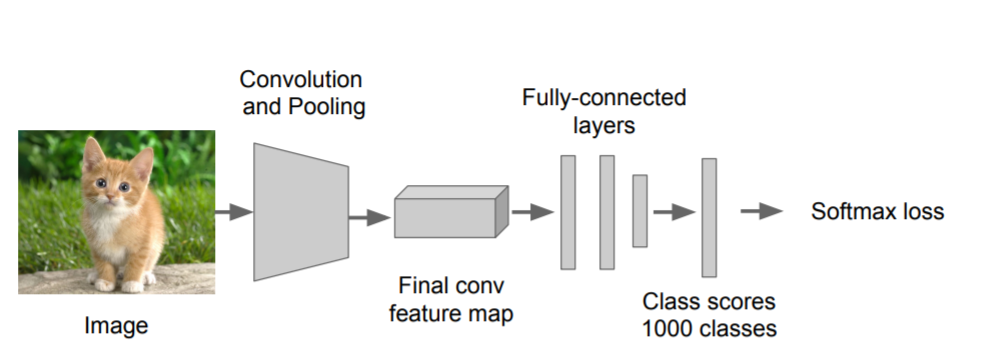
\includegraphics[width=0.8\columnwidth]{images/chap2/rcnn_1.png}
	    \footcaption{Sử dụng một mô hình mạng VGG-16 có sẵn là bộ phân loại 1000 class}
	    \label{fig:2.28}
	    \end{figure}
	\end{center}
	\footnotetext{Nguồn: \url{http://cs231n.stanford.edu/slides/2016/winter1516_lecture8.pdf}}
    \item Sau đó huấn luyện lại layer FC cuối cùng để tính các regions và features của vật thể cần phân loại
    \begin{center}
    	\begin{figure}[H]
	    \centering
	    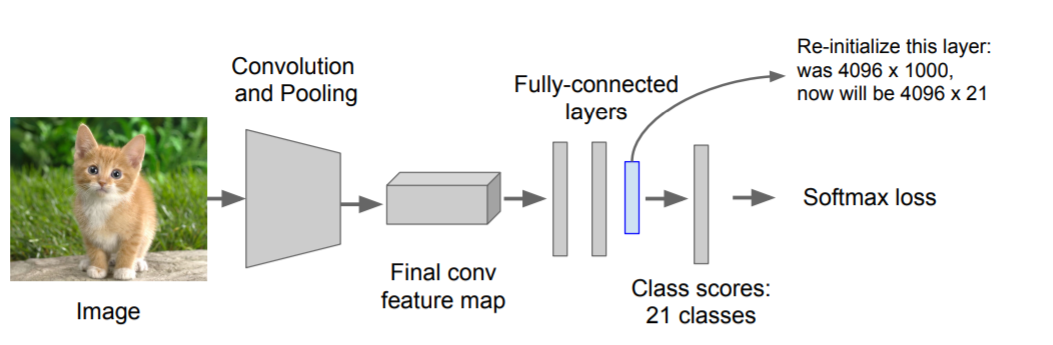
\includegraphics[width=0.8\columnwidth]{images/chap2/rcnn_2.png}
	    \footcaption{Thay lớp fully-connected cuối cùng bằng lớp fully-connected mới với số lượng class mới}
	    \label{fig:2.29}
	    \end{figure}
	\end{center}
	\footnotetext{Nguồn: \url{http://cs231n.stanford.edu/slides/2016/winter1516_lecture8.pdf}}
	Ở hình \ref{fig:2.29}, thay vì dùng 1000 loại, nếu chúng ta chỉ cần phân loại 20 loại thì ta điều chỉnh lớp fully-connected cuối cùng từ $4096 \times 1000$ thành $4096 \times 21$ (20 loại + 1 loại là background, hình ví dụ bên trên), với 4096 là chiều dài của một vector trong lớp fully-connected. Ta bỏ đi lớp fully-connected cuối cùng, lớp được dùng để đưa ra kết quả phân loại 1000 loại, và thay bằng lớp fully-connected cho ra kết quả phân loại là 21 loại. Tiến hành huấn luyện cho mô hình mạng này để đạt được bộ trọng số thích hợp.
    \item Bước này là bước trích xuất đặc trưng của ảnh, ở đây nó lấy tất cả proposal được trích xuất ra từ trong ảnh (xấp xỉ 2000 proposals một ảnh), thay đổi kích cỡ cho phù hợp với đầu vào của CNN rồi dùng CNN chạy feed forward để lấy được các đặc trưng của ảnh sau đó lưu lại.
    \begin{center}
    	\begin{figure}[H]
	    \centering
	    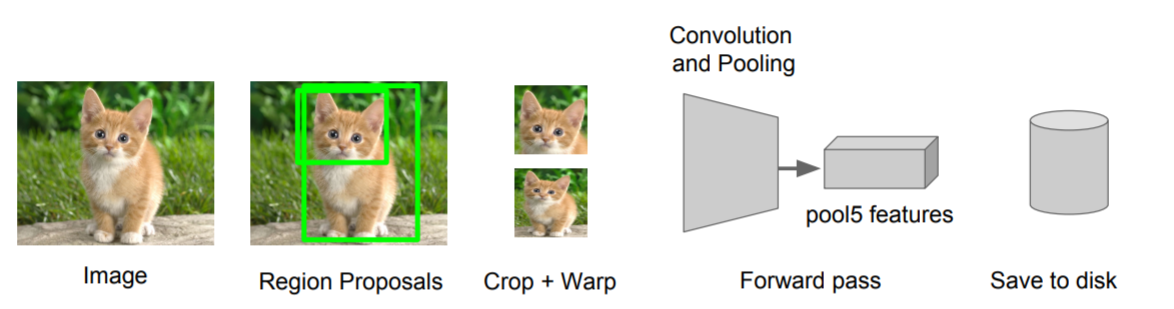
\includegraphics[width=0.8\columnwidth]{images/chap2/rcnn_3.png}
	    \footcaption{Trích xuất đặc trưng của các region proposal}
	    \label{fig:2.30}
	    \end{figure}
	\end{center}
	\footnotetext{Nguồn: \url{http://cs231n.stanford.edu/slides/2016/winter1516_lecture8.pdf}}
	Các region proposal được tìm thấy nhờ sử dụng thuật toán selective search \cite{uijlings2013selective}.
	
	Mỗi proposal được đưa vào mô hình mạng để trích xuất ra được đặc trưng ở cuối các lớp convolutional (Hình \ref{fig:2.30}). Lưu ý rằng bộ dữ liệu nè sẽ có kích thước rất lớn nên cần được lưu trữ vào một vùng nhớ có kích thước lớn.
    \item Huấn luyện SVM phân loại các đặc trưng là thuộc loại nào (với mỗi lớp dùng một SVM nhị phân)
    \begin{center}
    	\begin{figure}[H]
	    \centering
	    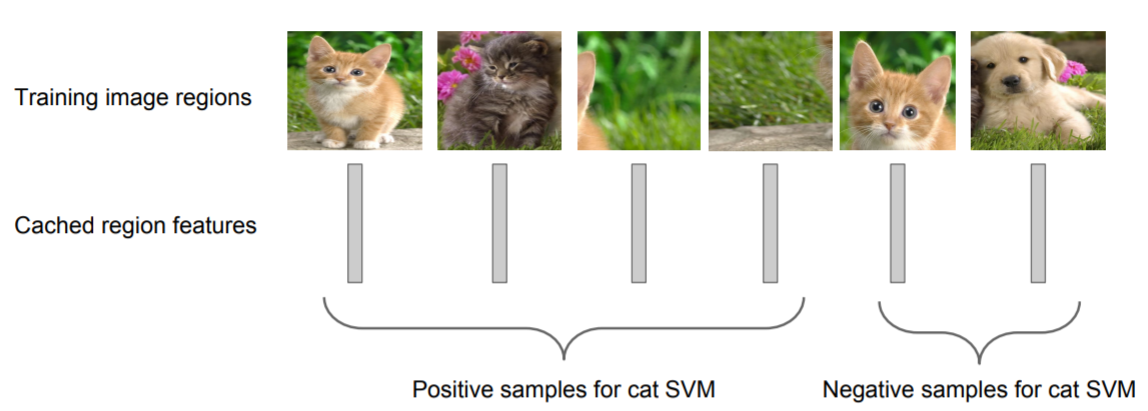
\includegraphics[width=0.8\columnwidth]{images/chap2/rcnn_4_1.png}
	    \footcaption{SVM phân loại cho cat và không phải cat}
	    \label{fig:2.31}
	    \end{figure}
	\end{center}
	\footnotetext{Nguồn: \url{http://cs231n.stanford.edu/slides/2016/winter1516_lecture8.pdf}}
    \begin{center}
    	\begin{figure}[H]
	    \centering
	    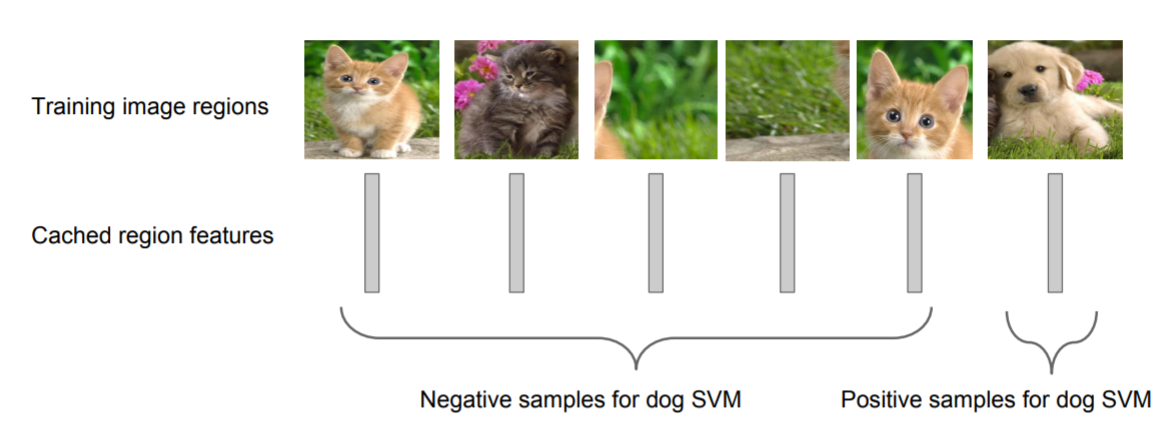
\includegraphics[width=0.8\columnwidth]{images/chap2/rcnn_4.png}
	    \footcaption{SVM phân loại cho dog và không phải dog}
	    \label{fig:2.32}
	    \end{figure}
	\end{center}
	\footnotetext{Nguồn: \url{http://cs231n.stanford.edu/slides/2016/winter1516_lecture8.pdf}}
	Hình \ref{fig:2.31} và \ref{fig:2.32} thể hiện cho hai loại SVM được dùng, một loại để phân biệt có phải cat hay không, một loại dùng để phân biệt có phải dog hay không.
    \item Huấn luyện Linear Regression model để hiệu chỉnh tọa độ các đỉnh của bounding boxes
    \begin{center}
    	\begin{figure}[H]
	    \centering
	    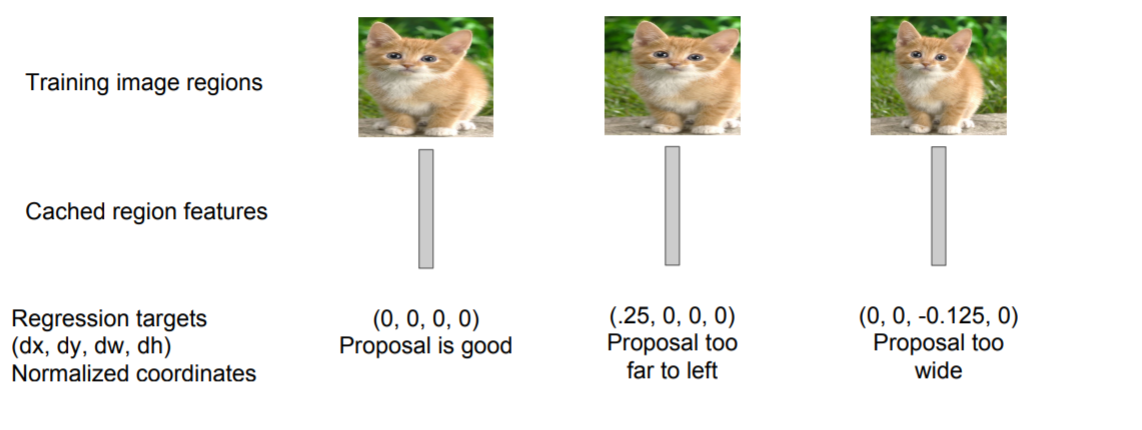
\includegraphics[width=0.8\columnwidth]{images/chap2/rcnn_5.png}
	    \footcaption{Thay lớp fully-connected cuối cùng bằng lớp fully-connected mới}
	    \label{fig:2.33}
	    \end{figure}
	\end{center}
	\footnotetext{Nguồn: \url{http://cs231n.stanford.edu/slides/2016/winter1516_lecture8.pdf}}
	Tọa độ của bounding box dự đoán ra sẽ được so sánh với dữ liệu được gán nhãn, từ đó tính lỗi và cập nhật lại trọng số (Hình \ref{fig:2.33}).
\end{enumerate}
R-CNN là một môn hình có khá nhiều khuyết điểm:
\begin{itemize}
	\item Thời gian chạy test chậm vì cần phải chạy forward cho tất cả các region proposal
	\item Đặc trưng và trọng số của các lớp trong CNN không được cập nhật khi huấn luyện ở những bước sử dụng các SVMs và regressors
	\item Quá trình huấn luyện phức tạp và phải qua nhiều bước.
\end{itemize}
\subsection{Fast R-CNN}
\subsubsection{Kiến trúc của Fast R-CNN}
	Để khắc phục những nhược điểm của mô hình R-CNN, mô hình cải tiến của nó - Fast R-CNN đã ra đời \cite{girshick2015fast}. \\
Mô hình này có những ưu điểm so với mô hình R-CNN:
\begin{itemize}
	\item Cho độ chính xác được đánh giá theo mAP (mean Average Precision) cao hơn so với R-CNN
	\item Quá trình huấn luyện chỉ với một bước duy nhất, với nhiều hàm lỗi khác nhau
	\item Quá trình huấn luyện cập nhật lại trọng số cho tất cả các lớp mạng
	\item Không cần lưu trữ những đặc trưng tìm được vào đĩa
\end{itemize}
Fast R-CNN dùng thuật toán Selective Search để có được các region proposals (sẽ mất thời gian bởi thuật toán cho ra hàng ngàn proposals với mỗi ảnh). Các proposals này sau đó được đưa tới layer RoI Pooling để thay đổi thành cùng một kích thước (hình \ref{chap2:2.34}).  

\begin{center}
    \begin{figure}[H]
    \centering
    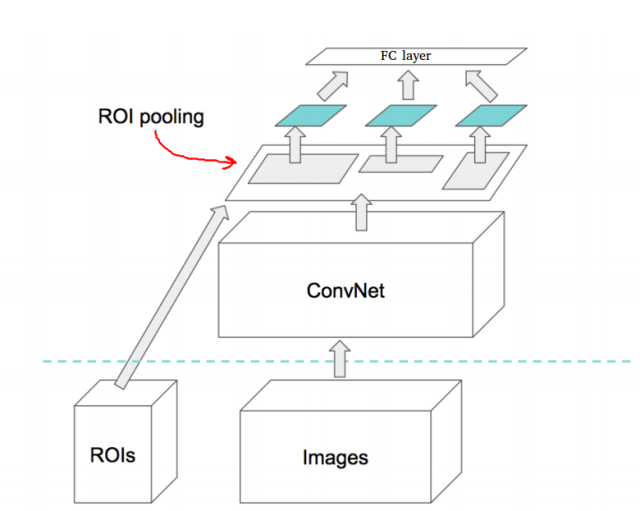
\includegraphics[width=0.6\columnwidth]{images/chap2/RoiPoolingLayer.png}
    \footcaption{Roi Pooling layer dùng để resize các proposals}
    \label{chap2:2.34}
    \end{figure}
\end{center}
\footnotetext{Nguồn: \url{http://cs231n.stanford.edu/slides/2016/winter1516_lecture8.pdf}}

Mô hình Fast R-CNN được huấn luyện theo các bước như sau:
\begin{enumerate}
    \item Sử dụng các mạng huấn luyện có sẵn
    \item Mô hình chỉ cần feed-forward một lần qua các lớp convolutional đối với ảnh đầu vào là đã thu được các features của nó.
    \item Tính toán vị trí của các features dựa vào kích thước và vị trí của các proposals đối với ảnh gốc để đưa ra các RoI 
    \item Dự đoán tọa độ các đỉnh của bounding box và vật thể nằm trong nó bằng các feature trong proposal.
\end{enumerate}

Đối với Fast R-CNN, do chia sẻ tính toán giữa các region trong ảnh, tốc độ thực thi của giải thuật đã được giảm đáng kể. Phần tốn nhiều chi phí nhất chính là phần đưa ra các region proposals đầu vào.

\begin{center}
    \begin{figure}[htp]
    \centering
    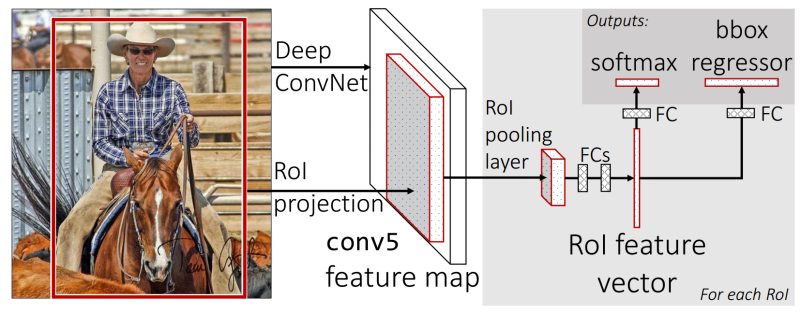
\includegraphics[width=0.5\columnwidth]{images/chap2/Fast_RCNN.png}
    \footcaption{Quá trình huấn luyện theo Fast R-CNN: hình ảnh đầu vào được đưa qua CNN huấn luyện sẵn để tạo thành feature map, các region proposals được xác định trên feature map để đưa ra các RoI, sau đó tiến hành phân loại và xác định bounding box từ các RoI đó}
    \label{fig:2.35}
    \end{figure}
\end{center}
\footnotetext{Nguồn: \cite{girshick2015fast}}
\subsubsection{Lớp RoI Pooling}
Lớp RoI Pooling dùng max pooling để chuyển những đặc trưng trong mỗi RoI trở thành một feature map nhỏ với một không gian 2 chiều cố định $h \times w$, với h và w là những hyper-parameter không phụ thuộc vào kích cỡ của RoI \cite{girshick2015fast}.

Lớp RoI Pooling hoạt động bằng cách chia RoI window với $h \times w$ thành  $H \times W$ ô sub-windows với kích thước xấp xỉ $H\mathbin{/}h \times W\mathbin{/}w$ và sau đó sử dụng max pooling giá trị ở mỗi sub-window để cho ra kích thước $h \times w$.

Hình \ref{chap2:cat1}, \ref{chap2:cat2}, \ref{chap2:cat3}, \ref{chap2:cat4} lần lượt là các bước hoạt động của RoI Pooling.
\begin{center}
    \begin{figure}[H]
    \centering
    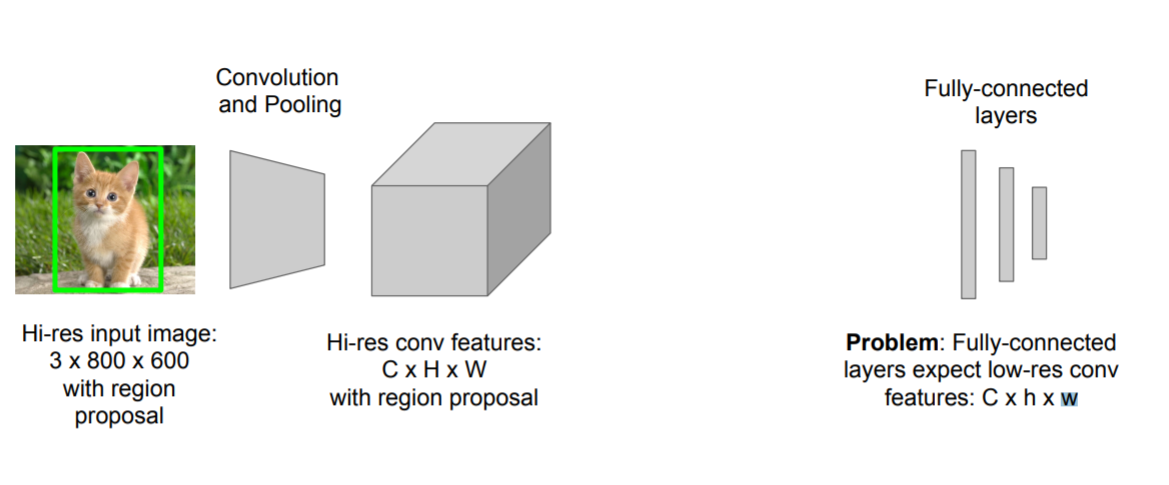
\includegraphics[width=0.8\columnwidth]{images/chap2/fastRCNN_1.png}
    \footcaption{Region Proposal được xác định}
    \label{chap2:cat1}
    \end{figure}
    \footnotetext{Nguồn: \url{http://cs231n.stanford.edu/slides/2016/winter1516_lecture8.pdf}}
\end{center}
\footnotetext{Nguồn: \url{http://cs231n.stanford.edu/slides/2016/winter1516_lecture8.pdf}}
\begin{center}
    \begin{figure}[H]
    \centering
    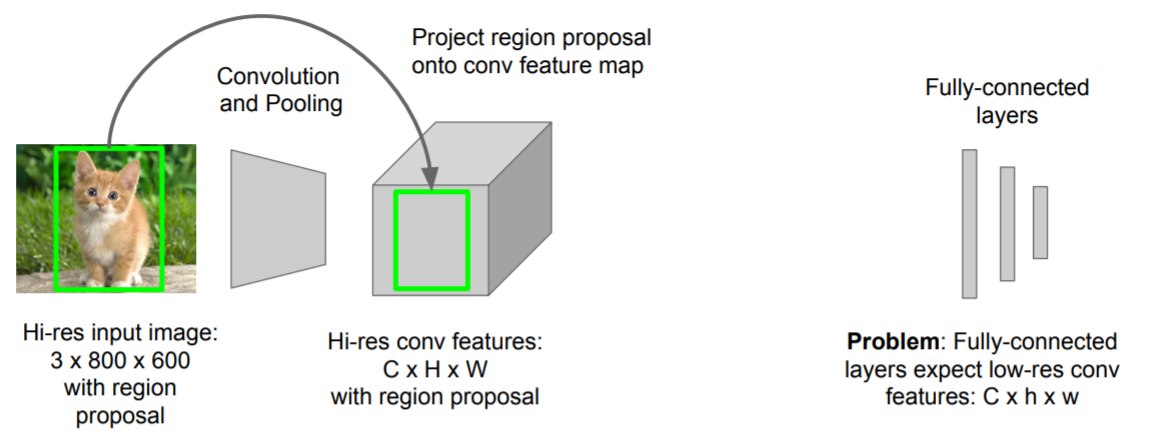
\includegraphics[width=0.8\columnwidth]{images/chap2/fastRCNN_2.png}
    \footcaption{Xác định Region Proposal trên feature map}
    \label{chap2:cat2}
    \end{figure}
\end{center}
\footnotetext{Nguồn: \url{http://cs231n.stanford.edu/slides/2016/winter1516_lecture8.pdf}}
\begin{center}
    \begin{figure}[H]
    \centering
    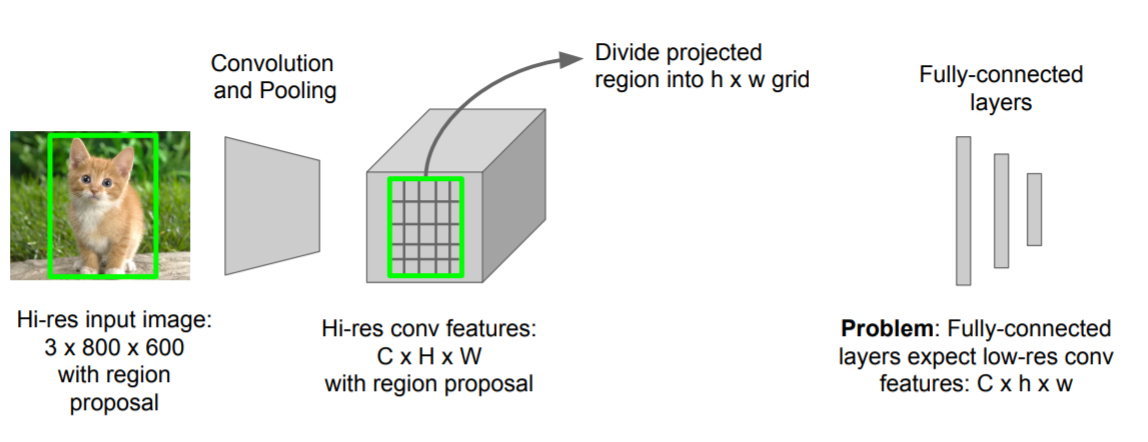
\includegraphics[width=0.8\columnwidth]{images/chap2/fastRCNN_3.png}
    \footcaption{Chia RoI window $H \times W$ xuống cỡ $h \times w$}
    \label{chap2:cat3}
    \end{figure}
\end{center}
\footnotetext{Nguồn: \url{http://cs231n.stanford.edu/slides/2016/winter1516_lecture8.pdf}}
\begin{center}
    \begin{figure}[H]
    \centering
    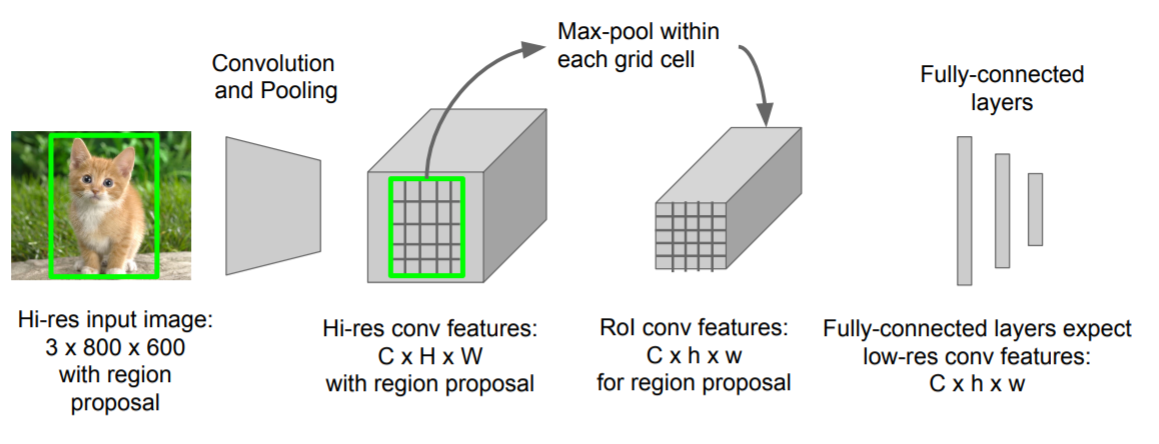
\includegraphics[width=0.8\columnwidth]{images/chap2/fastRCNN_4.png}
    \footcaption{Thực hiện max pooling}
    \label{chap2:cat4}
    \end{figure}
\end{center}
\footnotetext{Nguồn: \url{http://cs231n.stanford.edu/slides/2016/winter1516_lecture8.pdf}}
\subsubsection{Các hàm lỗi}
Fast R-CNN có hai lớp output đó là lớp tính xác suất phân bố $\mathbin{p} = (p_0, ..., p_K)$ trên mỗi RoI, với $K + 1$ loại. Thông thường xác suất $p$ sẽ được tính bởi hàm softmax thông qua $\mathbin{K} + 1$  outputs của lớp fully-connected. Lớp output thứ hai sẽ cho các thông số hồi quy của bounding box, $t^k = (t_x^k, t_y^k, t_w^k, t_h^k)$ với $\mathbin{k}$ là số chỉ mục của vật thể, $x, y, w, h$ lần lượt là tọa độ trục x, y, chiều dài, chiều cao của bounding box.

Trong quá trình huấn luyện, mỗi RoI đều được gán nhãn với một lớp ground-truth $\mathbin{u}$ và một ground-truth bounding-box $v$. Hàm lỗi $L$ cho mỗi RoI đã gán nhãn được xác định như sau:
\begin{center}
\begin{equation}
	L(p, u, t^u, v) = L_{cls}(p, u) + \lambda[u\geq 1]{L_{loc}}(t^u, v),
\end{equation}
\end{center}
Trong đó: 

$L_{cls}(p, u) = -\log p_u$ là log loss của class true $u$.

$p$ là xác suất phân bố của K + 1 classes

$u$ là ground-truth class $u$

$v$ là tọa độ ground-truth box

$t^u$ là tọa độ của bounding box thuộc class $u$

$L_{cls}$ là hàm lỗi của classifier

$L_{loc}$ là hàm lỗi của regressor

~\\
Hàm lỗi ${L_{loc}}$ được đặc tả qua bounding box true $v = (v_x, v_y, v_w, v_h)$ và kết quả dự đoán $t^u = (t_x^u, t_y^u, t_w^u, t_h^u)$. Điều kiện $[u\geq 1]$ bằng 1 khi $u \geq 1$ và bằng 0 nếu ngược lại, ý nghĩa của nó là nếu loại u có chỉ mục là 0 (là vùng nền, không chứa vật thể) thì sẽ không cần học vị trí của nó. \\
Tham số $\lambda$ được sử dụng để giữ cân bằng giữa hai hàm lỗi. Thông thường $\lambda$ sẽ có giá trị là 1.
Công thức hồi quy để tìm bounding box:
\begin{center}
\begin{equation}
	L_{loc}(t^u, v) = \sum_{i\in \{ x,y,w,h \}}smooth_{L_1}(t_i^u - v_i),
\end{equation}
\end{center}	
\begin{center}
\begin{equation}
    \text{với } smooth_{L_1}(x)=
    \begin{cases}
      0.5x^2, & \text{nếu}\ |a| < 1 \\
      |x| - 0.5, & \text{ngược lại,}
    \end{cases}
  \end{equation}
\end{center}
Hàm lỗi $L_1$ ít bị ảnh hưởng bởi các outliers hơn hàm lỗi $L_2$ được dùng trong mô hình R-CNN. Việc huấn luyện với hàm lỗi $L2$ cần phải chọn lọc tham số và learning rate một cách kĩ lưỡng để tránh việc gradients bị sai.
\subsection{Faster R-CNN}
Mặc dù đã được cải tiến nhiều nhưng Fast R-CNN vẫn còn một khuyết điểm rất lớn đó chính là sử dụng một mô hình thuật toán khác (selective search) để tìm ra các region proposals, việc này tạo ra hiệu ứng thắt cổ chai vì quá trình tìm kiếm các region proposals này diễn ra còn khá chậm. Vì thế mô hình Faster R-CNN tiếp tục được đưa ra giải quyết được khuyết điểm về thời gian thực thi của hai giải thuật trên bằng cách huấn luyện một mô hình hiệu quả hơn và thay thế vai trò của các thuật toán như Selective Search vốn rất chậm chạp.

Ý tưởng chính của giải thuật là dùng lớp Convolutional cuối cùng để dự đoán region proposals thay cho giải thuật selective search của mô hình Fast R-CNN cũ. Dựa vào hình \ref{faster_rcnn}, Faster R-CNN bao gồm hai modules:
\begin{enumerate}
    \item RPN (Region Proposals Network): đưa ra tập hợp các proposals dựa vào lớp Convolutional cuối cùng
    \item Fast R-CNN Roi Pooling: Phân loại và xác định vị trí từng proposals.
\end{enumerate}
\begin{center}
    \begin{figure}[H]
    \centering
    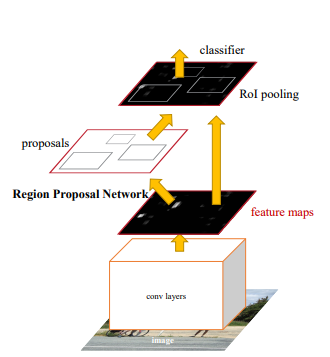
\includegraphics[width=0.7\columnwidth]{images/chap2/Faster_Rcnn_1.png}
    \footcaption{Quá trình huấn luyện theo Faster R-CNN}
    \label{chap2:faster_rcnn}
    \end{figure}
\end{center}
\footnotetext{Nguồn: \cite{ren2015faster}}
\subsubsection{Region Proposals Network}
Region Proposals Network lấy một hình với kích thước bất kì làm dữ liệu đầu vào và trả ra một tập tọa độ các proposals, với region là một khung hình chữ nhật.

Cách tạo ra các region proposals là cho trượt một sliding window (hình \ref{chap2:sliding_window}) nhỏ (một mô hình mạng nhỏ) $n \times n$ trên feature map. Sliding window này sẽ chuyển dữ liệu đầu vào thành những feature có kích thước rất nhỏ, thường là $1 \times 1$. Những feature này sẽ được đưa vào hai lớp fully-connected khác nhau. Một lớp là classifier dùng để phân loại đồng thời tính ra xác suất loại đó của feature đưa vào. Lớp còn lại là một regressor để tìm ra tọa độ bounding box.
\begin{center}
	\begin{figure}[H]
	\centering
	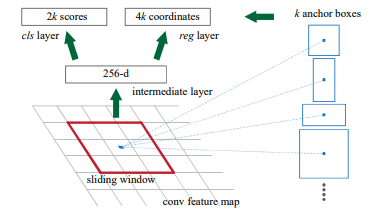
\includegraphics[width=0.7\columnwidth]{images/chap2/rpn.png}
    \footcaption{Sliding window}
    \label{chap2:sliding_window}
	\end{figure}
\end{center}
\footnotetext{Nguồn: \cite{ren2015faster}}

Ở mỗi vị trí của sliding window, giả sử có $k$ proposal được tìm thấy, khi đó regressor sẽ có $4k$ dữ liệu được xuất ra, tương ứng cho 4 tọa độ cho mỗi bounding box của proposal. Mỗi classifier cho hai loại score, một loại dự đoán xác suất cho trường hợp có vật và loại còn lại thì ngược lại. Những cái $k$ proposal được đề cập ở trên được gọi là anchors. Thường thì sẽ có 9 anchors  gồm hình tứ giác có 3 tỉ lệ với 3 kích thước khác nhau cho mỗi cho mỗi vị trí của sliding window trong feature map. Các anchor này sẽ được phân loại là có chứa vật hoặc không dựa trên tỉ lệ Intersection over Union sẽ được trình bày ở phần sau. Nếu tỉ lệ IoU này lớn hơn 0.7 thì anchor sẽ được cho là có chứa vật, ngược lại nếu IoU nhỏ hơn 0.3 thì anchor sẽ được cho là không chứa vật. Nếu 0.3 < IoU < 0.7 thì anchor đó sẽ được bỏ qua. Phương pháp này gọi là Non-Max Suppression. Dựa vào những anchor này, mô hình có thể có được xác suất chứa vật của mỗi region proposal tương ứng với một anchor đến ground-truth box tương ứng để xác định vị trí của bounding box.

Hàm lỗi:
\begin{center}
	\begin{equation}
		L(\{p_i\},\{y_i\}) = \frac{1}{N_{cls}}\sum_{i}L_{cls}(p_i, p_i^{*}) + \lambda \frac{1}{N_{reg}} \sum_{i}p_i^{*}L_{reg}(t_i, t_i^{*})
	\end{equation}
\end{center}
Trong đó:

$i$ là chỉ mục của anchor trong mini-batch

$p_i$ là xác suất dự đoán anchor thứ $i$ là vật thể

giá trị của ground-truth $p_i^*$ là 1 hoặc 0

$t_i$ là tọa độ bounding box dự đoán của anchor thứ $i$

$t_i^*$ là tọa độ ground-truth box
~\\
Các hyper-parameter $N_{cls}$, $N_{reg}$ và $\lambda$được dùng để chuẩn hóa lại công thức hàm lỗi trên. Theo bài báo \cite{ren2015faster}, $N_{cls}$ có giá trị bằng với kích thước của mini-batch và $N_{reg}$ được xấp xỉ bằng số lượng anchor chạy trên feature map.

\subsubsection{Huấn luyện Regional Proposals Network}
\begin{enumerate}
    \item Chọn một mạng CNN đã được train
    \item Từ layer Convolutional cuối cùng, ta được feature maps (hình \ref{chap2:last_convo})
    \begin{center}
    \begin{figure}[H]
    \centering
    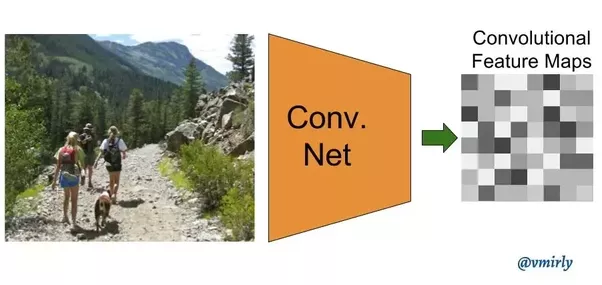
\includegraphics[width=0.7\columnwidth]{images/chap2/step-1.png}
    \footcaption{Feed-forward ảnh đầu vào thu được các features}
    \label{chap2:last_convo}
    \end{figure}
    \end{center}
    \footnotetext{Nguồn: \url{https://www.quora.com/How-does-the-region-proposal-network-RPN-in-Faster-R-CNN-work}}
    \item Với feature có được ở bước trước, ta dùng một sliding window, với mỗi bước trượt, ta tạo k anchors (trong hình \ref{chap2:anchor_9} là 9), với các tỉ lệ đa dạng (hình vuông, $1 \times 2$, $2 \times 1$, ...)\\
    \begin{center}
    \begin{figure}[H]
    \centering
    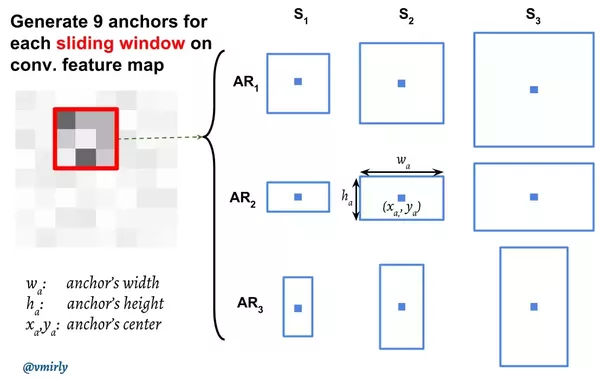
\includegraphics[width=0.7\columnwidth]{images/chap2/step-2.png}
    \footcaption{Tạo 9 anchors với từng sliding window }
    \label{chap2:anchor_9}
    \end{figure}
    \end{center}
    \footnotetext{Nguồn: \url{https://www.quora.com/How-does-the-region-proposal-network-RPN-in-Faster-R-CNN-work}}
    \item Huấn luyện một RPN với đầu vào là output của bước 3 có hai tác dụng chính: dự đoán tọa độ của bounding box và dự đoán bounding box đó có chứa vật thể hay không. Hình \ref{chap2:good_anchor} là một ví dụ về các anchors cho kết quả khá tốt
    \begin{center}
    \begin{figure}[H]
    \centering
    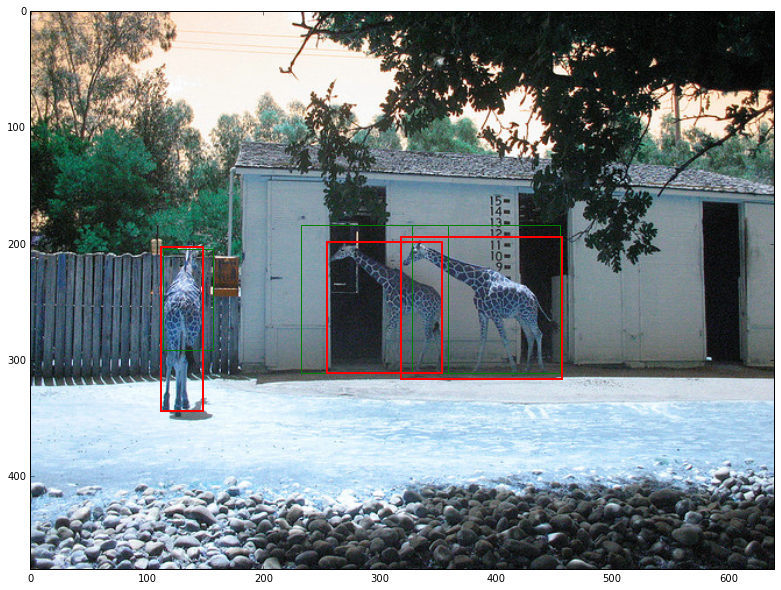
\includegraphics[width=0.7\columnwidth]{images/chap2/index.png}
    \footcaption{Những anchor có overlap khá tôt. Màu đỏ là ground truth boxes, màu xanh là anchor được tạo ra }
    \label{chap2:good_anchor}
    \end{figure}
    \end{center}
    \footnotetext{Nguồn: \url{https://www.quora.com/How-does-the-region-proposal-network-RPN-in-Faster-R-CNN-work}}
\end{enumerate}
\subsubsection{Mô hình mạng Faster R-CNN}
\begin{center}
    \begin{figure}[H]
    \centering
    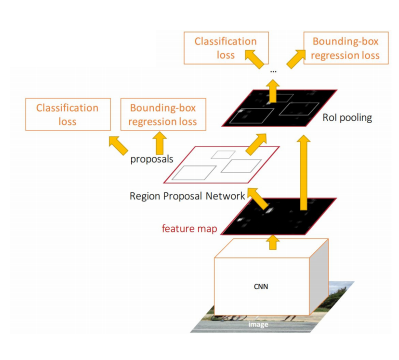
\includegraphics[width=0.7\columnwidth]{images/chap2/Faster_Rcnn_3.png}
    \footcaption{Mô hình huấn luyện Faster R-CNN}
    \label{chap2:faster_rcnn}
    \end{figure}
\end{center}
\footnotetext{\cite{ren2015faster}}
Nhờ lớp RPN, mô hình giải thuật Faster R-CNN trở nên nhanh hơn vì không còn bị thắt nút chai do phải dùng giải thụật khác để tìm ra các proposals. Các proposal này cùng với feature map được đưa vào quá trình RoI Pooling áp dụng theo giải thuật Fast R-CNN (hình \ref{chap2:faster_rcnn}), vậy mô hình Faster R-CNN gồm có tổng cộng 4 hàm lỗi:
\begin{itemize}
	\item Lỗi RPN classification
	\item Lỗi RPN regression
	\item Lỗi Fast R-CNN classification
	\item Lỗi Fast R-CNN regression
\end{itemize}
\section{Các phương pháp kiểm tra}
\subsection{Intersection over Union}
Trong bài toán nhận diện vật thể sử dụng 4 tọa độ để xác định bounding box, Intersection over Union (IoU) là một phương pháp thường được áp dụng để xét xem vật thể nhận diện được đã đúng với dữ liệu đươc gán nhãn chưa. Cần có hai cặp tọa độ để áp dụng phương pháp này, đó là tọa độ của bounding box nhận diện được và tọa độ của ground-truth box được gán nhãn sẵn một cách thủ công, thường bởi con người, dùng để kiểm tra vị trí của bounding box nhận diện được đã chính xác chưa.

Trong thực tế đối với vấn đề nhận diện ảnh, rất khó để có phương pháp so sánh trực tiếp các tọa độ $(x, y)$ nhận diện được trong ảnh bởi thuật toán xem có trùng với các tọa độ $(x, y)$ trong ground-truth box hay không. Do đó kĩ thuật đánh giá dựa trên sự chồng lên nhau (overlapping) được đề xướng và áp dụng thực tiễn.

Công thức tính IoU:

\begin{center}
	\begin{equation}
		IoU = \frac{\text{diện tích } \text{bounding box } \cap \text{ground-truth box}}{\text{diện tích } \text{bounding box } \cup \text{ground-truth box}}
	\end{equation}
\end{center}

IoU thường được tính bằng tỉ lệ diện tích vùng giao (intersection) giữa bounding box với ground-truth box so với diện tích vùng hợp (union) giữa ground-truth box và bounding box (hình \ref{chap2:iou_cal}). Từ đó ta có thể thấy được tỉ lệ chồng lên nhau của hai box.

\begin{center}
\begin{figure}[H]
    \centering
    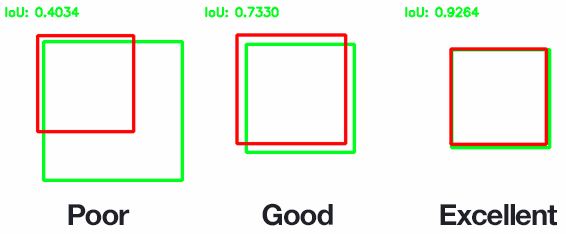
\includegraphics[width=0.7\columnwidth]{images/chap2/iou.png}
    \footcaption{Ví dụ về kĩ thuật đánh giá áp dụng IoU}
    \label{chap2:iou_cal}
    \end{figure}
\end{center}
\footnotetext{Nguồn: https://www.pyimagesearch.com/2016/11/07/intersection-over-union-iou-for-object-detection/}

Với những kết quả bounding box nhận diện được chồng nhiều lên ground-truth box thì IoU sẽ có giá trị cao và ngược lại, nếu kết quả bounding box quá nhỏ hay quá lớn so với ground-truth box thì IoU sẽ có giá trị thấp.

\subsection{Image matching}
Đây là phương pháp so sánh vật thể nhận diện được trong ảnh với vật thể đã gán nhãn của chính ảnh đó để đánh giá độ chính xác của giải thuật.\\
Theo \cite{szeliski2010computer}:
\begin{itemize}
	\item TP: True Positive
	
	Là những trường hợp vật thể được nhận diện đúng với vật thể được gán nhãn.
	\item FN: False Negative
	
	Là những trường hợp không nhận diện được vật thể nhưng vật thể đó được gán nhãn.	
	\item FP: False Positive
	
	Là những trường hợp nhận diện được vật thể nhưng vật thể đó không có thực trong nhãn.
	\item TN: True Negative
	
	Là những trường hợp không nhận diện được vật thể và vật thể không có thực trong nhãn.
\end{itemize}
\subsection{Precision và recall}
Công thức của precision và recall như sau:
\begin{center}
	\begin{equation}
		Precision = \frac{\text{true positives}}{\text{true positives } + \text{ false positives}}
	\end{equation}
\end{center}
\begin{center}
	\begin{equation}
		Recall = \frac{\text{true positives}}{\text{true positives } + \text{ false negatives}}
	\end{equation}
\end{center}
Precision được xem là thước đo để đánh giá độ chính xác của những khẳng định từ giải thuật. $TP + FP$ là tất cả những trường hợp giải thuật cho kết quả là positive, đối với bài toán nhận diện vật thể thì nó có nghĩa là tất cả các trường hợp giải thuật nhận diện là có vật thể. Vậy precision đại diện cho tỉ lệ chính xác của những phán đoán của giải thuật cho rằng vị trí nào có vật thể. Ví dụ Precision có giá trị là 0.8, mà thuật toán tìm được 5 vị trí có vật thể, vậy có nghĩa là có 4 vị trí là chính xác so với dữ liệu gán nhãn.

Recall thì được xem là thước đo để đánh giá độ chính xác so với dữ liệu được gán nhãn. $TP + FN$ là tất cả những trường hợp được gán nhãn là positive. Độ đo này chủ yếu để xác định độ chính xác hoặc sự tìm ra đầy đủ của giải thuật. Điều này áp dụng vào bài toán nhận diện vật thể có nghĩa là recall giúp ta đánh giá xem một giải thuật có thật sự nhận diện đủ các mẫu được gán nhãn hay không.

Khi sử dụng hai tỉ lệ này để đánh giá độ chính xác cân phải xem xét sự phù hợp của bài toán, nếu quá thiên về precision thì recall sẽ thấp, có nghĩa là nếu quá tập trung vào việc mỗi vật dự đoán ra từ giải thuật phải chính xác thì sẽ có rất nhiều trường hợp bị thiếu và ngược lại nếu tập trung vào recall thì precision sẽ thấp, có nghĩa là nếu cứ tập trung quá vào việc nhận diện đủ các vật thể so với dữ liệu gán nhãn thì những vật bị nhận diện thừa sẽ tăng lên.
